\documentclass[11pt,a4paper]{article}

\usepackage{amsfonts,amssymb,amsmath}
\usepackage[margin=1in]{geometry}
\usepackage[none]{hyphenat}
\usepackage{graphicx}
\usepackage{fancyhdr}
\usepackage{float}
\usepackage{color}
\usepackage{xcolor}
\usepackage{tikz}
\usepackage{polynom}
\usepackage{bigints}
\usepackage{esint}
\usepackage[nottoc,notlot,notlof]{tocbibind}

\usetikzlibrary{quotes,angles,graphs,patterns,fadings,arrows.meta,shapes,trees,bending}

% grad, div and curl are operator NAMES. Set as bare letters in maths they come
% out italic, so "grad" reads as the product g.r.a.d - the same defect as a bare
% \cos. These give them upright type and the correct spacing.
\DeclareMathOperator{\grad}{grad}
\DeclareMathOperator{\dive}{div}
\DeclareMathOperator{\curl}{curl}

\parindent 0ex
\setlength{\parskip}{0.55\baselineskip}
% Displays carry their own skips; with a non-zero \parskip on top of them,
% consecutive displays drift apart. Tighten them so a derivation reads as one
% argument rather than as a column of disconnected formulae.
\setlength{\abovedisplayskip}{0.5\baselineskip}
\setlength{\belowdisplayskip}{0.5\baselineskip}
\setlength{\abovedisplayshortskip}{0.25\baselineskip}
\setlength{\belowdisplayshortskip}{0.25\baselineskip}

\pagestyle{fancy}
\fancyfoot[C]{\thepage}
\fancyhead{}
\fancyhead[R]{\rightmark}
\renewcommand{\headrulewidth}{0pt}

% Theorem environments. The source declared none: its 125 examples, 91
% solutions, 21 definitions and 30 theorems were set as red bold text with the
% number typed by hand, so LaTeX numbered nothing and inserting an example meant
% renumbering the rest of the subsection.
\usepackage{amsthm}
\theoremstyle{definition}
% One shared counter running section.subsection.n, as in the other courses here.
\newtheorem{thm}{Theorem}[subsection]
\newtheorem{defn}[thm]{Definition}
\newtheorem{exa}[thm]{Example}
\newtheorem{prop}[thm]{Proposition}
\newtheorem{coro}[thm]{Corollary}
\newtheorem{lem}[thm]{Lemma}
\newtheorem{result}[thm]{Result}
\newtheorem{exe}[thm]{Exercise}
\newtheorem*{note}{Note}
\newtheorem*{remark}{Remark}
\newtheorem{problemx}{Problem}[subsection]
\newenvironment{problem}{\begin{problemx}}{\end{problemx}}
\newenvironment{solution}
  {\renewcommand{\qedsymbol}{}\begin{proof}[\textit{Solution}.]}
  {\end{proof}}
\usepackage{enumitem}
% A heading that is legal inside a theorem body, a list or a float, where
% \subsubsection is not. Same weight as \subsubsection* so the two read alike.
\newcommand{\subhead}[1]{%
  \par\medskip\noindent\textbf{#1}\par\nobreak\smallskip}


% Time series notation.
\DeclareMathOperator{\Var}{Var}
\DeclareMathOperator{\Cov}{Cov}
\DeclareMathOperator{\Corr}{Corr}

\begin{document}
% Title page depersonalised for the web, as with every other course here.
% The identity kept below is the autocorrelation function, which is what makes a
% time series a subject of its own rather than a sample of independent points.
\begin{titlepage}
\thispagestyle{empty}
\begin{center}
\vspace*{3cm}
{\Huge\bfseries Time Series Analysis}\\[1.2cm]
{\large Lecture Notes}\\[2.5cm]
\line(1,0){300}\\[1.5cm]
$$\rho(\tau) = \frac{\gamma(\tau)}{\gamma(0)},
\qquad \gamma(\tau) = \Cov\left(X_t,\,X_{t+\tau}\right)$$
\end{center}
\end{titlepage}

\tableofcontents
\thispagestyle{empty}
\clearpage
\setcounter{page}{1}


\title{\textbf{TIME SERIES ANALYSIS}}
\author{NEPHAT JESHURUN MWANZA}
\maketitle

\begin{center}
\hrulefill
\end{center}

\section{Introduction}
\begin{defn}
A \textbf{time series} is an ordered sequence of observations $x_1, x_2, \dots, x_n$. The ordering is usually in
time, but it may be in another dimension, such as distance along a line.
\end{defn}

What makes a time series a subject of its own is that its observations are \emph{dependent}: this month's
value is related to last month's. In most of statistics observations are assumed independent, and their order
does not matter; in a time series the order is the most important thing about the data. Time series arise in
every field:
\begin{itemize}
\item \textbf{Agriculture}: annual crop production, livestock numbers, crop prices.
\item \textbf{Business and economics}: annual sales of a product, commodity prices, price indices such as
inflation, stock-exchange earnings, exchange rates.
\item \textbf{Engineering}: electrical signals, voltage, sound.
\item \textbf{Geophysics}: the height of ocean waves, seismic records.
\item \textbf{Meteorology}: sea-surface temperature, rainfall, wind speed.
\item \textbf{Medicine}: annual mortality rates, failure rates of a surgical procedure.
\item \textbf{Quality control}: measurements monitoring a production process.
\item \textbf{Social sciences}: birth rates, mortality rates, accident and crime rates.
\end{itemize}

\subsection{Types of time series}
\begin{enumerate}
\item A time series recorded continuously in time is said to be \textbf{continuous}, for example an electrical
signal or a voltage trace.
\item A time series recorded only at specific times, usually equally spaced, is said to be \textbf{discrete}, for
example a monthly interest rate, an annual crop yield or a daily closing price.
\end{enumerate}
A discrete series may arise by \emph{sampling} a continuous one at intervals (the temperature at noon each
day) or by \emph{aggregating} over intervals (the rainfall in each month). These notes deal with discrete series
observed at equal intervals, written $x_t$ for $t = 1, \dots, n$.

\subsection{Objectives of time-series analysis}
A major objective is to understand and describe the mechanism that generates the series. Because the
observations are dependent, this mechanism can be exploited for:
\begin{enumerate}
\item \textbf{Description}: computing descriptive measures, and above all plotting the series, to characterise its
main features.
\item \textbf{Explanation}: when observations are taken on two or more variables, using the variation in one
series to explain the variation in another, for example rainfall and crop yield.
\item \textbf{Prediction}: forecasting future values from the past of the series.
\item \textbf{Control}: adjusting a process, especially in quality control in manufacturing, so that it stays on
target.
\end{enumerate}

\section{Descriptive techniques}
Simple descriptive methods are the first step of any analysis. They classify the main properties of a series,
and often suggest the model to use.

\subsection{Components of a time series}
Traditionally a series is analysed by \emph{decomposing} it into components, each a source of variation:
\begin{enumerate}
\item \textbf{Trend}: a long-term change in the mean level.
\item \textbf{Seasonal effects}: variation that repeats with a fixed period, usually annual, such as sales that
rise every December.
\item \textbf{Cyclic effects}: variation with a longer, less regular period, from some other physical or economic
cause; business cycles, for example, often have a period of five to seven years.
\item \textbf{Irregular fluctuations}: what is left when the trend, seasonal and cyclic variation have been
removed. These residuals may or may not be random.
\end{enumerate}
The components are usually combined in one of two ways. With trend $m_t$, seasonal effect $s_t$ and irregular term
$\varepsilon_t$:
\[
\text{additive:}\quad x_t = m_t + s_t + \varepsilon_t , \qquad\qquad \text{multiplicative:}\quad x_t = m_t\,s_t\,\varepsilon_t .
\]
In the additive model the seasonal swings have the same size whatever the level of the series; in the
multiplicative model they grow in proportion to the level. Figure~\ref{fig:ts-components} shows how the
components add up to a series.

\begin{figure}[H]
\centering
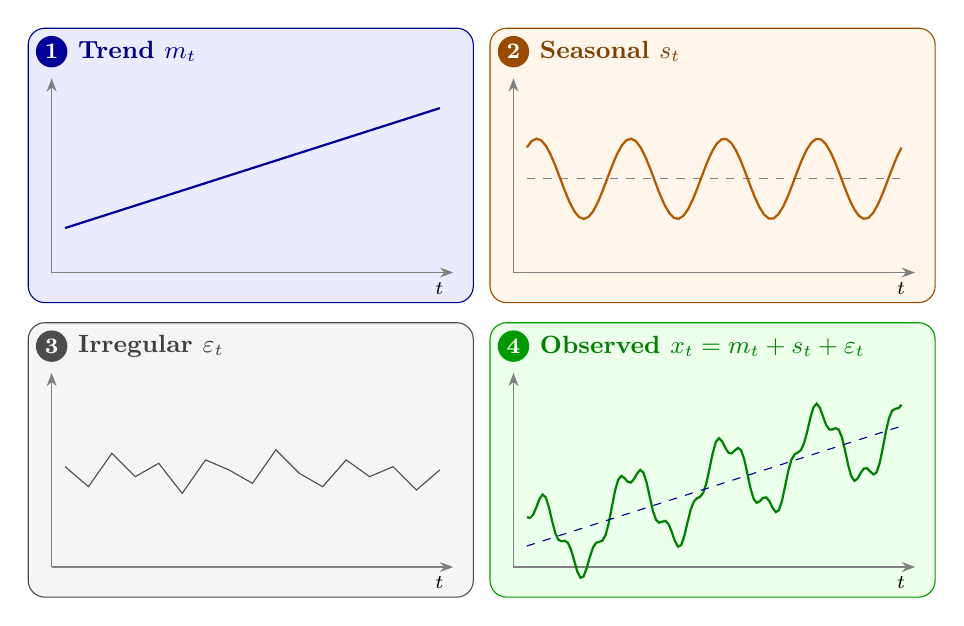
\begin{tikzpicture}[scale=0.85]
\foreach \px/\py/\col/\num/\name in {
 0/4.4/blue/1/{Trend $m_t$},
 6.9/4.4/orange/2/{Seasonal $s_t$},
 0/0/gray/3/{Irregular $\varepsilon_t$},
 6.9/0/green/4/{Observed $x_t = m_t + s_t + \varepsilon_t$}} {
 \begin{scope}[shift={(\px,\py)}]
  \filldraw[fill=\col!8,draw=\col!60!black,rounded corners=6pt] (-0.35,-0.45) rectangle (6.3,3.65);
  \node[circle,fill=\col!60!black,text=white,inner sep=1.5pt,font=\footnotesize\bfseries] at (0,3.3) {\num};
  \node[anchor=west,font=\small\bfseries,text=\col!50!black] at (0.25,3.3) {\name};
  \draw[-Stealth,gray] (0,0) -- (6.0,0) node[below left,black,font=\scriptsize] {$t$};
  \draw[-Stealth,gray] (0,0) -- (0,2.9);
  \ifnum\num=1
   \draw[-,thick,blue!60!black] plot[domain=0.2:5.8,samples=30] (\x,{0.6+0.32*\x});
  \fi
  \ifnum\num=2
   \draw[-,dashed,gray] (0.2,1.4) -- (5.8,1.4);
   \draw[-,thick,orange!70!black] plot[domain=0.2:5.8,samples=80] (\x,{1.4+0.6*sin(\x*360/1.4)});
  \fi
  \ifnum\num=3
   \draw[-,gray!60!black] plot coordinates {(0.2,1.5) (0.55,1.2) (0.9,1.7) (1.25,1.35) (1.6,1.55) (1.95,1.1) (2.3,1.6) (2.65,1.45) (3.0,1.25) (3.35,1.75) (3.7,1.4) (4.05,1.2) (4.4,1.6) (4.75,1.35) (5.1,1.5) (5.45,1.15) (5.8,1.45)};
  \fi
  \ifnum\num=4
   \draw[-,thick,green!50!black] plot[domain=0.2:5.8,samples=120] (\x,{0.25+0.32*\x+0.6*sin(\x*360/1.4)+0.15*sin(\x*977)});
   \draw[-,dashed,blue!60!black] plot[domain=0.2:5.8,samples=30] (\x,{0.25+0.32*\x});
  \fi
 \end{scope}
}
\end{tikzpicture}
\caption{The components of an additive time series. The observed series (panel~4) is the sum of a trend, a
seasonal pattern and irregular fluctuations; its trend is shown dashed.}
\label{fig:ts-components}
\end{figure}

\subsection{Plotting the series and stationarity}
The first and most important step in any time-series analysis is to plot the observations against time. The
plot shows the important features of the series, such as trend, seasonality, outliers and sudden changes
(discontinuities), and it helps in formulating a sensible model.

Loosely, a series is \textbf{stationary} if it has no systematic change in mean (no trend), no systematic change in
variance, and no strictly periodic variation. Most of the theory of later sections is for stationary series, so a
common strategy is to remove the trend and seasonal effects first and then model what is left. Stationarity is
defined precisely in the next section.

\subsection{Transformations}
A plot may suggest transforming the series, for example by taking logarithms or square roots. There are three
main reasons:
\begin{enumerate}
\item to stabilise the variance;
\item to make the seasonal effect additive;
\item to make the data closer to normally distributed.
\end{enumerate}
The logarithm does the first two jobs at once when the series is multiplicative, as the next result shows.

\begin{prop}\label{prop:ts-log}
\begin{enumerate}[label=(\roman*)]
\item If $x_t = m_t\,s_t\,\varepsilon_t$ with all factors positive, then $\log x_t = \log m_t + \log s_t + \log\varepsilon_t$, an additive model.
\item If the standard deviation of $x_t$ is proportional to its mean $\mu_t$, say $\operatorname{sd}(x_t) = c\,\mu_t$, then approximately
$\Var(\log x_t) \approx c^2$, which does not depend on $t$.
\end{enumerate}
\end{prop}

\begin{proof}
(i) is the rule $\log(abc) = \log a + \log b + \log c$. For (ii), by Taylor's theorem $\log x_t \approx \log\mu_t + (x_t - \mu_t)/\mu_t$ when $x_t$ is
close to $\mu_t$. The right-hand side has variance $\Var(x_t)/\mu_t^2 = c^2\mu_t^2/\mu_t^2 = c^2$.
\end{proof}

So when the seasonal swings, or the scatter, of a series grow with its level, take logarithms first.

\subsection{Estimating and removing the trend}
There are two broad approaches: estimate the trend and subtract it, or remove it by differencing.

\subhead{Fitting a curve}
A simple trend can be fitted by least squares as a function of time, for example a straight line $m_t = a + bt$, a
quadratic, or an exponential growth curve $m_t = ae^{bt}$ (linear after taking logarithms). This gives a formula,
but it imposes one shape on the whole series.

\subhead{Moving averages}
A \textbf{moving average} smooths the series by replacing each value with an average of its neighbours. The
simple moving average of order $2q + 1$ is
\[
\hat m_t = \frac{1}{2q + 1}\sum_{j=-q}^{q} x_{t+j} , \qquad t = q + 1, \dots, n - q .
\]

\begin{prop}\label{prop:ma-linear}
A moving average $\sum_{j=-q}^{q} w_jx_{t+j}$ with weights that add to $1$ and are symmetric ($w_{-j} = w_j$) leaves a linear trend
unchanged: if $x_t = a + bt$, then $\sum_j w_jx_{t+j} = a + bt$.
\end{prop}

\begin{proof}
$\sum_j w_j(a + b(t + j)) = (a + bt)\sum_j w_j + b\sum_j jw_j = a + bt + 0$, since the terms $jw_j$ and $(-j)w_{-j}$ cancel in pairs.
\end{proof}

So a moving average keeps the trend while averaging out the irregular fluctuations, whose average over
several periods is close to zero. For seasonal data, the window should cover exactly one full season, so that
the seasonal effect is also averaged out. With quarterly data a season has $4$ observations, an even number,
so a simple average of four would be centred between two time points. The standard remedy is the
\textbf{centred moving average} (or $2\times4$ moving average):
\[
\hat m_t = \tfrac18x_{t-2} + \tfrac14x_{t-1} + \tfrac14x_t + \tfrac14x_{t+1} + \tfrac18x_{t+2} ,
\]
the average of the two four-term averages that straddle $t$. For monthly data the $2\times12$ average is built the
same way, with weights $\frac{1}{24}$ at the ends and $\frac{1}{12}$ in between.

\begin{prop}\label{prop:centred-ma}
Suppose $x_t = a + bt + s_t$, where $s_t$ has period $4$ ($s_{t+4} = s_t$) and $s_1 + s_2 + s_3 + s_4 = 0$. Then the centred moving average
gives $\hat m_t = a + bt$ exactly.
\end{prop}

\begin{proof}
The weights are symmetric and add to $\frac18 + \frac14 + \frac14 + \frac14 + \frac18 = 1$, so by Proposition~\ref{prop:ma-linear} the trend part
passes through unchanged. The seasonal part gives $\frac18s_{t-2} + \frac14s_{t-1} + \frac14s_t + \frac14s_{t+1} + \frac18s_{t+2}$. Since $s_{t+2} = s_{t-2}$, this is
$\frac14(s_{t-2} + s_{t-1} + s_t + s_{t+1})$, a quarter of the sum over four consecutive quarters, which is $0$.
\end{proof}

\subhead{Seasonal indices}
Once the trend has been estimated, the \emph{detrended} values $x_t - \hat m_t$ (additive model) contain the seasonal
effect plus noise. Averaging them over all the years for each season gives the raw seasonal indices, which
are adjusted, if necessary, to add to zero. Subtracting the indices from the data gives the \textbf{seasonally
adjusted} series. For a multiplicative model the same steps use ratios $x_t/\hat m_t$, and the indices are adjusted to
average $1$.

\begin{exa}\label{exa:quarterly}
The quarterly sales of a shop (in thousands) over four years were:
\begin{center}
\begin{tabular}{c|cccc}
Year & Q1 & Q2 & Q3 & Q4 \\
\hline
1 & 19 & 22 & 26 & 23 \\
2 & 22 & 26 & 30 & 26 \\
3 & 26 & 30 & 35 & 31 \\
4 & 31 & 36 & 40 & 35 \\
\end{tabular}
\end{center}
Estimate the trend by a centred moving average, find the seasonal indices of an additive model, and
seasonally adjust the series.
\end{exa}

\begin{solution}
\emph{The trend.} The centred moving average at $t$ is the sum of the two four-quarter totals that straddle $t$,
divided by $8$. The four-quarter totals, starting from quarters $1$--$4$, are
\[
90, \ 93, \ 97, \ 101, \ 104, \ 108, \ 112, \ 117, \ 122, \ 127, \ 133, \ 138, \ 142 .
\]
So the first centred average, at $t = 3$ (year~1, Q3), is $(90 + 93)/8 = 22.875$, the next is $(93 + 97)/8 = 23.75$, and so on:
\begin{center}
\begin{tabular}{ccrrr}
$t$ & Quarter & $x_t$ & $\hat m_t$ & $x_t - \hat m_t$ \\
\hline
3 & Y1 Q3 & 26 & 22.875 & 3.125 \\
4 & Y1 Q4 & 23 & 23.750 & $-0.750$ \\
5 & Y2 Q1 & 22 & 24.750 & $-2.750$ \\
6 & Y2 Q2 & 26 & 25.625 & 0.375 \\
7 & Y2 Q3 & 30 & 26.500 & 3.500 \\
8 & Y2 Q4 & 26 & 27.500 & $-1.500$ \\
9 & Y3 Q1 & 26 & 28.625 & $-2.625$ \\
10 & Y3 Q2 & 30 & 29.875 & 0.125 \\
11 & Y3 Q3 & 35 & 31.125 & 3.875 \\
12 & Y3 Q4 & 31 & 32.500 & $-1.500$ \\
13 & Y4 Q1 & 31 & 33.875 & $-2.875$ \\
14 & Y4 Q2 & 36 & 35.000 & 1.000 \\
\end{tabular}
\end{center}
No centred average exists for the first two or last two quarters.

\emph{Seasonal indices.} Averaging the detrended values quarter by quarter:
\begin{align*}
\text{Q1}: \ & (-2.750 - 2.625 - 2.875)/3 = -2.75 , \\
\text{Q2}: \ & (0.375 + 0.125 + 1.000)/3 = 0.50 , \\
\text{Q3}: \ & (3.125 + 3.500 + 3.875)/3 = 3.50 , \\
\text{Q4}: \ & (-0.750 - 1.500 - 1.500)/3 = -1.25 .
\end{align*}
These add to $-2.75 + 0.50 + 3.50 - 1.25 = 0$, so no adjustment is needed. Sales are $3.5$ thousand above trend in the third
quarter and $2.75$ thousand below it in the first.

\emph{Seasonally adjusted series.} Subtracting the indices,
\begin{center}
\begin{tabular}{c|cccc}
Year & Q1 & Q2 & Q3 & Q4 \\
\hline
1 & 21.75 & 21.50 & 22.50 & 24.25 \\
2 & 24.75 & 25.50 & 26.50 & 27.25 \\
3 & 28.75 & 29.50 & 31.50 & 32.25 \\
4 & 33.75 & 35.50 & 36.50 & 36.25 \\
\end{tabular}
\end{center}
The adjusted series rises steadily, by about one thousand a quarter, and shows that the jump from Q4 to Q1
each year is not a real fall in business but the seasonal pattern. Figure~\ref{fig:quarterly} shows the data and
the trend.
\end{solution}

\begin{figure}[H]
\centering
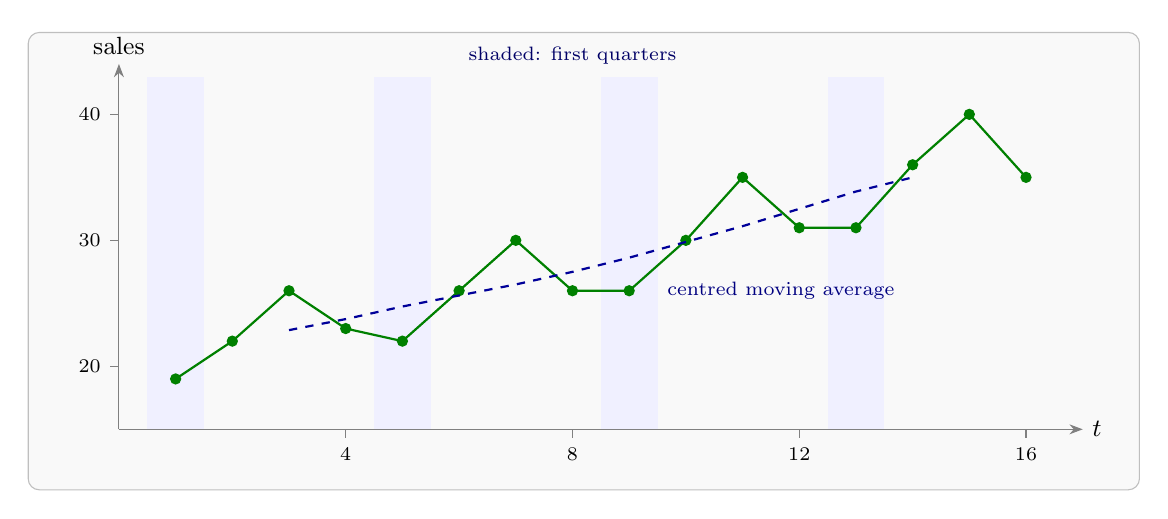
\begin{tikzpicture}[xscale=0.72,yscale=0.16]
\filldraw[fill=gray!5,draw=gray!50,rounded corners=4pt] (-1.6,10.2) rectangle (18.0,46.5);
\foreach \y in {1,...,4} \fill[blue!6] ({4*\y-3.5},15) rectangle ({4*\y-2.5},43);
\draw[-Stealth,gray] (0,15) -- (17,15) node[right,black,font=\small] {$t$};
\draw[-Stealth,gray] (0,15) -- (0,44) node[above,black,font=\small] {sales};
\foreach \t in {4,8,12,16} \draw[gray] (\t,15) -- (\t,14.3) node[below,black,font=\scriptsize] {\t};
\foreach \v in {20,30,40} \draw[gray] (0,\v) -- (-0.15,\v) node[left,black,font=\scriptsize] {\v};
\draw[-,thick,green!50!black] plot coordinates {(1,19) (2,22) (3,26) (4,23) (5,22) (6,26) (7,30) (8,26) (9,26) (10,30) (11,35) (12,31) (13,31) (14,36) (15,40) (16,35)};
\foreach \a/\b in {1/19,2/22,3/26,4/23,5/22,6/26,7/30,8/26,9/26,10/30,11/35,12/31,13/31,14/36,15/40,16/35}
 \fill[green!50!black] (\a,\b) circle (0.1 and 0.45);
\draw[-,thick,dashed,blue!60!black] plot coordinates {(3,22.875) (4,23.75) (5,24.75) (6,25.625) (7,26.5) (8,27.5) (9,28.625) (10,29.875) (11,31.125) (12,32.5) (13,33.875) (14,35)};
\node[font=\scriptsize,text=blue!50!black,anchor=north west] at (9.5,27.5) {centred moving average};
\node[font=\scriptsize,text=blue!40!black,anchor=south] at (8,43.2) {shaded: first quarters};
\end{tikzpicture}
\caption{The quarterly sales of Example~\ref{exa:quarterly} (solid) with the centred moving-average trend (dashed).
Every first quarter (shaded) dips below the trend and every third quarter rises above it.}
\label{fig:quarterly}
\end{figure}

\subhead{Differencing}
Instead of estimating the trend, it can be removed by \textbf{differencing}. The difference operator is
$\nabla x_t = x_t - x_{t-1}$, and the seasonal difference of period $s$ is $\nabla_sx_t = x_t - x_{t-s}$.

\begin{prop}\label{prop:differencing}
\begin{enumerate}[label=(\roman*)]
\item If $m_t = a + bt$, then $\nabla m_t = b$, a constant; if $m_t$ is a quadratic in $t$, then $\nabla^2m_t = \nabla(\nabla m_t)$ is a constant.
\item If $s_t$ has period $s$, then $\nabla_ss_t = 0$.
\end{enumerate}
\end{prop}

\begin{proof}
(i) $\nabla(a + bt) = (a + bt) - (a + b(t - 1)) = b$. For $m_t = a + bt + ct^2$, $\nabla m_t = b + c(2t - 1)$, which is linear in $t$, so a second difference
gives the constant $2c$. (ii) $\nabla_ss_t = s_t - s_{t-s} = 0$ by periodicity.
\end{proof}

Differencing is the basis of the ARIMA models of later sections. For the quarterly sales, the seasonal
differences $\nabla_4x_t$ are $3, 4, 4, 3, 4, 4, 5, 5, 5, 6, 5, 4$: the seasonal pattern has gone, and what remains varies around
the yearly growth of about $4$ (four quarters at one thousand each).

\subsection{The sample autocorrelation function}\label{ssec:sample-acf}
Sample autocorrelation coefficients are an important guide to the properties of a time series. They measure
the correlation between observations a given time apart.

Recall that for $n$ pairs of observations $(x_i, y_i)$, the correlation coefficient is
\[
r = \frac{\sum(x_i - \bar x)(y_i - \bar y)}{\sqrt{\sum(x_i - \bar x)^2\sum(y_i - \bar y)^2}} .
\]
Given $n$ observations $x_1, \dots, x_n$ of a time series, we can form the $n - 1$ pairs
\[
(x_1, x_2), \ (x_2, x_3), \ \dots, \ (x_{n-1}, x_n) ,
\]
and
treat the first member of each pair as one variable and the second as another. Their correlation is
\[
r_1 = \frac{\sum_{t=1}^{n-1}(x_t - \bar x_{(1)})(x_{t+1} - \bar x_{(2)})}{\sqrt{\sum_{t=1}^{n-1}(x_t - \bar x_{(1)})^2\sum_{t=1}^{n-1}(x_{t+1} - \bar x_{(2)})^2}} ,
\]
where $\bar x_{(1)}$ is the mean of the first $n - 1$ observations and $\bar x_{(2)}$ the mean of the last $n - 1$. For a long series both means
are close to the overall mean $\bar x$, and both sums of squares in the denominator are close to $\sum_{t=1}^n(x_t - \bar x)^2$. This
gives the simpler and standard form
\[
r_1 = \frac{\sum_{t=1}^{n-1}(x_t - \bar x)(x_{t+1} - \bar x)}{\sum_{t=1}^{n}(x_t - \bar x)^2} ,
\]
the \textbf{autocorrelation coefficient} at lag $1$. Similarly, the correlation between observations a
distance $k$ apart is the \textbf{autocorrelation coefficient at lag $k$},
\[
r_k = \frac{\sum_{t=1}^{n-k}(x_t - \bar x)(x_{t+k} - \bar x)}{\sum_{t=1}^{n}(x_t - \bar x)^2} .
\]
In practice the autocorrelations are calculated from the \textbf{sample autocovariance} at lag $k$,
\[
c_k = \frac1n\sum_{t=1}^{n-k}(x_t - \bar x)(x_{t+k} - \bar x) ,
\]
as $r_k = c_k/c_0$, for $k = 1, 2, \dots$, with $k < n$. (The divisor $n$ rather than $n - k$ is deliberate: it keeps the sequence of
$c_k$ a valid autocovariance function, a property needed in Section~3.)

\begin{prop}\label{prop:rk-bound}
$|r_k| \le 1$ for every $k$.
\end{prop}

\begin{proof}
Write $u_t = x_t - \bar x$. By the Cauchy--Schwarz inequality,
\[
\Bigl|\sum_{t=1}^{n-k}u_tu_{t+k}\Bigr| \le \sqrt{\sum_{t=1}^{n-k}u_t^2}\sqrt{\sum_{t=1}^{n-k}u_{t+k}^2} \le \sqrt{\sum_{t=1}^nu_t^2}\sqrt{\sum_{t=1}^nu_t^2} = \sum_{t=1}^nu_t^2 ,
\]
since each partial sum of squares is at most the full one. Dividing by $\sum u_t^2$ gives $|r_k| \le 1$.
\end{proof}

\subhead{The correlogram}
A plot of $r_k$ against $k$ is called a \textbf{correlogram}. It is one of the most useful descriptive tools, and
its shape is a strong clue to the nature of the series (Figure~\ref{fig:correlograms}):
\begin{enumerate}
\item \emph{Random series.} If the observations are independent, $r_k$ is approximately $N(0, 1/n)$ for each $k \ne 0$, so about $95\%$
of the coefficients should lie within $\pm2/\sqrt n$. (This result is justified later, with the partial autocorrelation function.)
\item \emph{Short-term correlation.} A fairly large $r_1$, followed by a few smaller positive coefficients that die
away towards zero, indicates that an observation above the mean tends to be followed by a few more.
\item \emph{Alternating series.} If successive observations tend to lie on opposite sides of the mean, the
correlogram alternates in sign, starting with a negative $r_1$.
\item \emph{Non-stationary series.} If the series has a trend, $r_k$ comes down only slowly and stays positive for large
lags: the trend dominates everything else. The correlogram is then of little use except to show that the
trend must be removed first.
\item \emph{Seasonal series.} If the series has a seasonal pattern, the correlogram oscillates with the same period:
for monthly data, large positive values at lags $12, 24, \dots$ and negative values around lags $6, 18, \dots$.
\end{enumerate}

\begin{figure}[H]
\centering
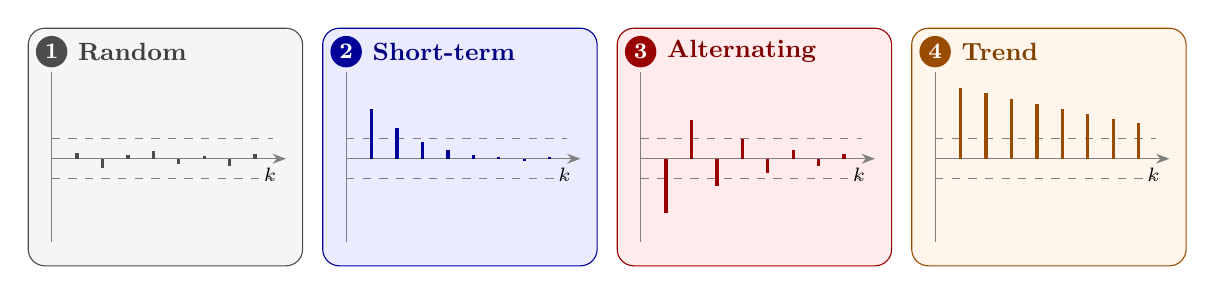
\begin{tikzpicture}[scale=0.85]
\foreach \px/\col/\num/\name/\vals in {
 0/gray/1/{Random}/{0.08,-0.12,0.05,0.1,-0.07,0.03,-0.1,0.06},
 4.4/blue/2/{Short-term}/{0.65,0.4,0.22,0.12,0.05,0.02,-0.03,0.02},
 8.8/red/3/{Alternating}/{-0.7,0.5,-0.36,0.25,-0.18,0.12,-0.09,0.06},
 13.2/orange/4/{Trend}/{0.92,0.85,0.78,0.71,0.64,0.58,0.52,0.46}} {
 \begin{scope}[shift={(\px,0)}]
  \filldraw[fill=\col!8,draw=\col!60!black,rounded corners=6pt] (-0.35,-1.6) rectangle (3.75,1.95);
  \node[circle,fill=\col!60!black,text=white,inner sep=1.5pt,font=\footnotesize\bfseries] at (0,1.6) {\num};
  \node[anchor=west,font=\small\bfseries,text=\col!50!black] at (0.25,1.6) {\name};
  \draw[-Stealth,gray] (0,0) -- (3.5,0) node[below left,black,font=\scriptsize] {$k$};
  \draw[-,gray] (0,-1.25) -- (0,1.3);
  \draw[-,dashed,gray] (0,0.3) -- (3.3,0.3);
  \draw[-,dashed,gray] (0,-0.3) -- (3.3,-0.3);
  \foreach \v [count=\k] in \vals
   \draw[-,very thick,\col!60!black] ({0.38*\k},0) -- ({0.38*\k},{1.15*\v});
 \end{scope}
}
\end{tikzpicture}
\caption{Typical correlograms at lags $1$ to $8$. Dashed lines: the band $\pm2/\sqrt n$. (1) A random series stays inside
the band. (2) Short-term correlation dies away quickly. (3) An alternating series alternates in sign. (4) A
series with a trend gives coefficients that decline only slowly.}
\label{fig:correlograms}
\end{figure}

\begin{exa}\label{exa:sample-acf}
Compute $r_1$, $r_2$ and $r_3$ for the series $4, 6, 9, 7, 5, 3, 4, 6, 8, 8$.
\end{exa}

\begin{solution}
Here $n = 10$ and $\bar x = 60/10 = 6$, so the deviations $u_t = x_t - 6$ are
\[
-2, \ 0, \ 3, \ 1, \ -1, \ -3, \ -2, \ 0, \ 2, \ 2 ,
\]
with $\sum u_t^2 = 4 + 0 + 9 + 1 + 1 + 9 + 4 + 0 + 4 + 4 = 36$. The lagged products are:
\begin{align*}
\text{lag } 1: \ & 0 + 0 + 3 - 1 + 3 + 6 + 0 + 0 + 4 = 15 , \\
\text{lag } 2: \ & -6 + 0 - 3 - 3 + 2 + 0 - 4 + 0 = -14 , \\
\text{lag } 3: \ & -2 + 0 - 9 - 2 + 0 - 6 - 4 = -23 .
\end{align*}
So
\[
r_1 = \frac{15}{36} = 0.417 , \qquad r_2 = \frac{-14}{36} = -0.389 , \qquad r_3 = \frac{-23}{36} = -0.639 .
\]
Equivalently, $c_0 = 36/10 = 3.6$ and $c_1 = 1.5$, giving $r_1 = 1.5/3.6$. The positive $r_1$ and the negative $r_3$ reflect the slow
up-and-down swing in the series, with a period of about six observations: values three apart tend to lie on
opposite sides of the mean. With only $10$ observations the band $\pm2/\sqrt{10} = \pm0.63$ is wide, and only $r_3$ reaches it.
\end{solution}

\subsection{Practice problems}
\begin{problem}\label{prob:ts-ma3}
Compute the simple moving average of order $3$ for the series $5, 8, 6, 9, 7, 10, 8$, and explain why it cannot be
computed at the first and last time points.
\end{problem}

\begin{solution}
The averages at $t = 2, \dots, 6$ are $(5 + 8 + 6)/3 = 6.33$, $(8 + 6 + 9)/3 = 7.67$, $(6 + 9 + 7)/3 = 7.33$, $(9 + 7 + 10)/3 = 8.67$ and
$(7 + 10 + 8)/3 = 8.33$. The series zig-zags, and the moving average smooths it into a gently rising trend. At $t = 1$ there is
no $x_0$, and at $t = 7$ no $x_8$, so the symmetric window does not fit.
\end{solution}

\begin{problem}\label{prob:ts-multiplicative}
Quarterly ratios $x_t/\hat m_t$ averaged over several years gave the raw multiplicative seasonal indices $0.90$, $1.05$, $1.20$,
$0.89$. Adjust them to average $1$, and seasonally adjust a third-quarter value of $48$.
\end{problem}

\begin{solution}
The raw indices add to $4.04$, an average of $1.01$, so divide each by $1.01$: $0.891$, $1.040$, $1.188$, $0.881$. The adjusted value
of the third-quarter observation is $48/1.188 = 40.4$: third quarters run about $19\%$ above trend.
\end{solution}

\begin{problem}\label{prob:ts-12ma}
Show that the $2\times12$ centred moving average has weights $\frac{1}{24}$ on $x_{t\pm6}$ and $\frac{1}{12}$ on $x_{t-5}, \dots, x_{t+5}$, and that it removes any
seasonal pattern of period $12$ whose effects add to zero.
\end{problem}

\begin{solution}
The two twelve-term averages straddling $t$ cover $x_{t-6}, \dots, x_{t+5}$ and $x_{t-5}, \dots, x_{t+6}$. Averaging them, $x_{t-5}, \dots, x_{t+5}$ appear in
both, with weight $\frac12(\frac1{12} + \frac1{12}) = \frac1{12}$, and $x_{t-6}$, $x_{t+6}$ in one only, with weight $\frac1{24}$. For the seasonal part,
$s_{t+6} = s_{t-6}$, so the weighted sum is $\frac1{12}(s_{t-6} + s_{t-5} + \dots + s_{t+5})$, a twelfth of the sum over a whole year, which is $0$.
\end{solution}

\begin{problem}\label{prob:ts-trend-acf}
For the series $x_t = t$, $t = 1, \dots, 10$, compute $r_1$ and $r_5$, and comment.
\end{problem}

\begin{solution}
$\bar x = 5.5$, and $u_t = t - 5.5$ runs from $-4.5$ to $4.5$ in steps of $1$, with $\sum u_t^2 = 82.5$. For lag $1$, $\sum_{t=1}^9u_tu_{t+1} = 57.75$, so
$r_1 = 0.70$. For lag $5$, $\sum_{t=1}^5u_tu_{t+5} = (-4.5)(0.5) + (-3.5)(1.5) + (-2.5)(2.5) + (-1.5)(3.5) + (-0.5)(4.5) = -21.25$, so $r_5 = -0.258$. The
coefficients of a short trending series fall steadily (here they turn negative because with $n = 10$ the two ends of the
series are paired); for a long trending series they stay positive and large for many lags. Either way the
correlogram mainly reflects the trend, which should be removed before the correlogram is interpreted.
\end{solution}

\section{Stochastic processes}
Time series are modelled as \emph{random processes}. A \textbf{stochastic process} is a family of random
variables $X(\omega, t)$ indexed by time $t$, where $\omega$ belongs to a sample space and $t$ to an index set (here the integers).
For a fixed $t$, $X(\omega, t)$ is a random variable. For a fixed $\omega$, $X(\omega, t)$ as a function of $t$ is called a \emph{sample
function} or a \textbf{realisation}. The population of all possible realisations is called the \emph{ensemble}.
An observed time series is thus one realisation of a stochastic process, and the aim of the analysis is to
learn about the process from that single realisation. We write $X_t$ for $X(\omega, t)$.

A process is described completely by the joint distributions of every finite set of its variables: for any
times $t_1, \dots, t_n$, the joint distribution function $F(x_{t_1}, \dots, x_{t_n})$ of $X_{t_1}, \dots, X_{t_n}$. This is usually far more than can be
known, and a simpler description uses the first and second moments:
\begin{itemize}
\item the \textbf{mean function} $\mu(t) = E(X_t)$;
\item the \textbf{variance function} $\sigma^2(t) = \Var(X_t) = E[(X_t - \mu(t))^2]$;
\item the \textbf{autocovariance function} $\gamma(t_1, t_2) = E[(X_{t_1} - \mu(t_1))(X_{t_2} - \mu(t_2))] = \Cov(X_{t_1}, X_{t_2})$.
\end{itemize}
The variance function is the special case $\sigma^2(t) = \gamma(t, t)$.

\subsection{Strict stationarity}
A process is \emph{first-order stationary} if the distribution of $X_t$ is the same for every $t$: $F(x_{t_1}) = F(x_{t_1+k})$ for all $t_1$, $k$. It is
\emph{second-order stationary in distribution} if $F(x_{t_1}, x_{t_2}) = F(x_{t_1+k}, x_{t_2+k})$ for all $t_1, t_2, k$, and \emph{$n$th-order stationary} if
\[
F(x_{t_1}, x_{t_2}, \dots, x_{t_n}) = F(x_{t_1+k}, x_{t_2+k}, \dots, x_{t_n+k})
\]
for all $t_1, \dots, t_n$ and $k$.

\begin{defn}
A process is \textbf{strictly stationary} if it is $n$th-order stationary for every $n = 1, 2, \dots$: the joint distribution of
$X_{t_1}, \dots, X_{t_n}$ is the same as that of $X_{t_1+k}, \dots, X_{t_n+k}$ for every $t_1, \dots, t_n$ and every shift $k$.
\end{defn}

In words, shifting the time origin by any amount $k$ has no effect on the distributions.

\begin{prop}\label{prop:strict-moments}
If $\{X_t\}$ is strictly stationary with finite variance, then
\begin{enumerate}[label=(\roman*)]
\item $\mu(t) = \mu$ and $\sigma^2(t) = \sigma^2$ are constants;
\item $\gamma(t_1, t_2)$ depends only on the lag $t_2 - t_1$.
\end{enumerate}
\end{prop}

\begin{proof}
(i) With $n = 1$, every $X_t$ has the same distribution, hence the same mean and variance. (ii) With $n = 2$, $(X_{t_1}, X_{t_2})$ has
the same joint distribution as $(X_{t_1+k}, X_{t_2+k})$ for every $k$. Taking $k = -t_1$, it is the same as that of $(X_0, X_{t_2-t_1})$, so its
covariance is a function of $t_2 - t_1$ alone.
\end{proof}

So for a stationary process we write $\gamma(k) = \Cov(X_t, X_{t+k})$, the \textbf{autocovariance at lag $k$}, and
\[
\rho(k) = \frac{\gamma(k)}{\gamma(0)} ,
\]
the \textbf{autocorrelation function} (ac.f.), which measures the correlation between $X_t$ and $X_{t+k}$. Here $\gamma(0) = \sigma^2$.

\subsection{Second-order stationarity}
Strict stationarity is a strong condition, and hard to check from data. In practice a weaker one is used.

\begin{defn}
A process is \textbf{second-order stationary} (or \textbf{weakly stationary}) if its mean is constant and its
autocovariance depends only on the lag:
\[
E(X_t) = \mu , \qquad \Cov(X_t, X_{t+k}) = \gamma(k) \quad\text{for all } t \text{ and } k ,
\]
with $\mu$ and $\gamma(0)$ finite.
\end{defn}

Taking $k = 0$, the variance $\gamma(0) = \sigma^2$ is also constant. Throughout these notes ``stationary'' means second-order
stationary unless stated otherwise. The two kinds are related as follows.

\begin{prop}\label{prop:strict-weak}
\begin{enumerate}[label=(\roman*)]
\item A strictly stationary process with finite variance is second-order stationary.
\item A second-order stationary process need not be strictly stationary.
\item A second-order stationary process is strictly stationary if, for every choice of times, its
variables have a multivariate normal joint distribution (a \emph{Gaussian process}).
\end{enumerate}
\end{prop}

\begin{proof}
(i) is Proposition~\ref{prop:strict-moments}. (ii) Let the $X_t$ be independent, with $X_t \sim N(0, 1)$ for odd $t$ and $X_t$ uniform on $(-\sqrt3, \sqrt3)$
for even $t$. Both distributions have mean $0$ and variance $1$, and different variables are uncorrelated, so $\mu = 0$ and
$\gamma(k) = 0$ for $k \ne 0$, $\gamma(0) = 1$: the process is second-order stationary. But $X_1$ and $X_2$ have different distributions, so it is not
first-order stationary. (iii) A multivariate normal distribution is determined by its mean vector and covariance
matrix. For a weakly stationary process, the mean vector of $(X_{t_1+k}, \dots, X_{t_n+k})$ is $(\mu, \dots, \mu)$ and its covariance matrix has entries
$\gamma(t_j - t_i)$, neither depending on $k$, so the joint distribution does not depend on $k$.
\end{proof}

\begin{exa}\label{exa:harmonic}
Let $X_t = A\cos(\lambda t) + B\sin(\lambda t)$, where $\lambda$ is a fixed frequency and $A$, $B$ are uncorrelated random variables with mean $0$
and variance $\sigma^2$. Show that $\{X_t\}$ is second-order stationary and find its ac.f.
\end{exa}

\begin{solution}
$E(X_t) = \cos(\lambda t)E(A) + \sin(\lambda t)E(B) = 0$. Since $\Cov(A, B) = 0$,
\begin{align*}
\Cov(X_t, X_{t+k}) &= \cos(\lambda t)\cos(\lambda(t + k))\Var(A) \\
&\qquad + \sin(\lambda t)\sin(\lambda(t + k))\Var(B) \\
&= \sigma^2\bigl[\cos(\lambda t)\cos(\lambda t + \lambda k) + \sin(\lambda t)\sin(\lambda t + \lambda k)\bigr] \\
&= \sigma^2\cos(\lambda k) ,
\end{align*}
by the identity $\cos a\cos b + \sin a\sin b = \cos(b - a)$. The mean is constant and the covariance depends only on $k$, so the
process is stationary, with $\gamma(0) = \sigma^2$ and $\rho(k) = \cos(\lambda k)$. Each realisation is a sinusoid with a random amplitude and
phase, and its correlations never die away: values a whole period apart are perfectly correlated. Processes
built from such components are the basis of the frequency-domain view in Section~\ref{sec:frequency}.
\end{solution}

\subsection{Properties of the autocorrelation function}
Suppose $\{X_t\}$ is stationary with mean $\mu$, variance $\sigma^2$, autocovariance $\gamma(k)$ and ac.f. $\rho(k)$. Then $\rho(k) = \gamma(k)/\gamma(0) = \gamma(k)/\sigma^2$,
and the following properties hold.

\begin{thm}\label{thm:acf-properties}
\begin{enumerate}[label=(\roman*)]
\item $\rho(0) = 1$.
\item The ac.f. is an even function: $\rho(-k) = \rho(k)$, and likewise $\gamma(-k) = \gamma(k)$.
\item $|\rho(k)| \le 1$ for every $k$.
\item $\gamma$ is \textbf{non-negative definite}: for any times $t_1, \dots, t_n$ and real numbers $a_1, \dots, a_n$,
\[
\sum_{i=1}^n\sum_{j=1}^n a_ia_j\gamma(t_i - t_j) \ge 0 .
\]
Equivalently, every matrix $\boldsymbol\Gamma_n$ with $(i, j)$ entry $\gamma(i - j)$ is non-negative definite.
\end{enumerate}
\end{thm}

\begin{proof}
(i) $\rho(0) = \gamma(0)/\gamma(0) = 1$.

(ii) By stationarity, $\gamma(-k) = \Cov(X_t, X_{t-k}) = \Cov(X_{t-k}, X_t)$, and shifting time by $k$ gives $\Cov(X_t, X_{t+k}) = \gamma(k)$.

(iii) For either sign, $0 \le \Var(X_t \pm X_{t+k}) = \sigma^2 + \sigma^2 \pm 2\gamma(k) = 2\sigma^2(1 \pm \rho(k))$, so $1 + \rho(k) \ge 0$ and $1 - \rho(k) \ge 0$.

(iv) The left-hand side is $\Var\bigl(\sum_ia_iX_{t_i}\bigr)$, since
$\Var(\sum_ia_iX_{t_i}) = \sum_i\sum_ja_ia_j\Cov(X_{t_i}, X_{t_j}) = \sum_i\sum_ja_ia_j\gamma(t_j - t_i)$, and $\gamma(t_j - t_i) = \gamma(t_i - t_j)$ by (ii). A variance is never negative.
\end{proof}

Property (iv) is a real restriction. Not every even function with $\rho(0) = 1$ and $|\rho(k)| \le 1$ is the ac.f. of some
stationary process, and (iv) is the test. Its most usable form is that all the matrices $\mathbf{R}_n = \boldsymbol\Gamma_n/\sigma^2$, with entries
$\rho(i - j)$, must have non-negative determinants.

Note also that the ac.f. does not determine the process. Different processes can have the same ac.f.; an
example appears in Section~\ref{sec:invertibility}, on invertibility. And a process with a trend or with a changing variance has
no ac.f. in this sense at all, which is why trend and seasonality are removed before the correlogram is used to
choose a model.

\begin{exa}\label{exa:not-acf}
Can $\rho(0) = 1$, $\rho(\pm1) = 0.8$ and $\rho(k) = 0$ for $|k| \ge 2$ be the autocorrelation function of a stationary process?
\end{exa}

\begin{solution}
The function is even, with $\rho(0) = 1$ and $|\rho(k)| \le 1$, so (i)--(iii) of Theorem~\ref{thm:acf-properties} hold. Check (iv) with $n = 3$:
\begin{align*}
\det\mathbf{R}_3 &= \det\begin{pmatrix} 1 & 0.8 & 0 \\ 0.8 & 1 & 0.8 \\ 0 & 0.8 & 1 \end{pmatrix} \\
&= 1(1 - 0.64) - 0.8(0.8 - 0) = 0.36 - 0.64 = -0.28 < 0 .
\end{align*}
So $\mathbf{R}_3$ has a negative eigenvalue, and there are weights $a_1, a_2, a_3$ for which $\Var(a_1X_1 + a_2X_2 + a_3X_3)$ would be negative.
For instance $\mathbf{a} = (1, -1, 1)$ gives $\mathbf{a}^\top\mathbf{R}_3\mathbf{a} = 3 - 4(0.8) = -0.2$. The function is not an ac.f. Intuitively, if $X_1$ and $X_2$ are
strongly correlated, and $X_2$ and $X_3$ are too, then $X_1$ and $X_3$ cannot be uncorrelated. (Section~\ref{sec:ma} shows that a
function of this shape is an ac.f. exactly when $|\rho(1)| \le \frac12$.)
\end{solution}

\section{Purely random process}
\subsection{Definition and properties}
\begin{defn}
A discrete process $\{Z_t\}$ is \textbf{purely random} if it consists of a sequence of mutually independent
random variables, all with the same distribution, with mean $\mu$ and variance $\sigma_Z^2$.
\end{defn}

\begin{prop}\label{prop:white-noise}
A purely random process is strictly stationary, with
\[
\gamma(k) = \begin{cases} \sigma_Z^2 , & k = 0 , \\ 0 , & k = \pm1, \pm2, \dots , \end{cases}
\qquad
\rho(k) = \begin{cases} 1 , & k = 0 , \\ 0 , & k = \pm1, \pm2, \dots \end{cases}
\]
\end{prop}

\begin{proof}
For any times $t_1, \dots, t_n$, the joint distribution of $Z_{t_1}, \dots, Z_{t_n}$ is the product of $n$ copies of the
common distribution, so it is unchanged by a shift. Independent variables are uncorrelated, so $\gamma(k) = 0$ for $k \ne 0$, and $\gamma(0) = \sigma_Z^2$.
\end{proof}

A purely random process is often called \textbf{white noise}; strictly, ``white noise'' only requires the
variables to be uncorrelated with constant mean and variance, which is enough for most of the theory. If the
$Z_t$ are also normal, independence and uncorrelatedness coincide, and the process is \emph{Gaussian white
noise}. White noise has no memory at all: knowing past values does not help to predict future ones. It is
important not for itself but as the building block from which the moving average, autoregressive and ARMA
processes of the following sections are constructed, usually with $\mu = 0$. Its correlogram is the benchmark
for a series with no structure: the sample autocorrelations are approximately $N(0, 1/n)$, as noted in
Section~\ref{ssec:sample-acf}.

\section{Random walk}
\subsection{Definition and properties}
\begin{defn}
Let $\{Z_t\}$ be a purely random process with mean $\mu$ and variance $\sigma_Z^2$. The process $\{X_t\}$ is a \textbf{random walk} if
\[
X_t = X_{t-1} + Z_t .
\]
\end{defn}

The process is usually started at $X_0 = 0$, so that $X_1 = Z_1$ and, by repeated substitution,
\[
X_t = Z_1 + Z_2 + \dots + Z_t = \sum_{i=1}^tZ_i .
\]
When $\mu \ne 0$ the process is a \emph{random walk with drift}. Random walks are standard models for share prices
and exchange rates: tomorrow's price is today's plus an unpredictable change.

\begin{thm}\label{thm:random-walk}
For the random walk started at $X_0 = 0$, and $1 \le s \le t$,
\begin{gather*}
E(X_t) = t\mu , \qquad \Var(X_t) = t\sigma_Z^2 , \\
\Cov(X_s, X_t) = s\sigma_Z^2 , \qquad \Corr(X_s, X_t) = \sqrt{s/t} .
\end{gather*}
The process is not stationary, but its first difference $\nabla X_t = X_t - X_{t-1} = Z_t$ is purely random.
\end{thm}

\begin{proof}
$E(X_t) = \sum_{i=1}^tE(Z_i) = t\mu$, and since the $Z_i$ are independent, $\Var(X_t) = \sum_{i=1}^t\Var(Z_i) = t\sigma_Z^2$. For $s \le t$,
\begin{align*}
\Cov(X_s, X_t) &= \Cov\Bigl(\sum_{i=1}^sZ_i, \ \sum_{j=1}^tZ_j\Bigr) = \sum_{i=1}^s\sum_{j=1}^t\Cov(Z_i, Z_j) \\
&= \sum_{i=1}^s\Var(Z_i) = s\sigma_Z^2 ,
\end{align*}
since only the terms with $i = j \le s$ are non-zero. Dividing by $\sqrt{s\sigma_Z^2 \cdot t\sigma_Z^2}$ gives the correlation. The variance grows with $t$ (and
the mean too, unless $\mu = 0$), so the process is not stationary; and $\nabla X_t = Z_t$ by definition.
\end{proof}

The correlation $\sqrt{s/t}$ depends on $s$ and $t$ separately, not just on their difference: $X_{10}$ and $X_{20}$ have correlation
$\sqrt{0.5} = 0.71$, while $X_{100}$ and $X_{110}$, also ten steps apart, have $\sqrt{100/110} = 0.95$. The paths wander further and
further from their starting point (Figure~\ref{fig:random-walk}), and the correlogram of an observed random walk
dies away only very slowly, like that of a series with a trend. Differencing turns it back into white noise:
this is the simplest example of the integrated models of Section~\ref{sec:integrated}.

\begin{figure}[H]
\centering
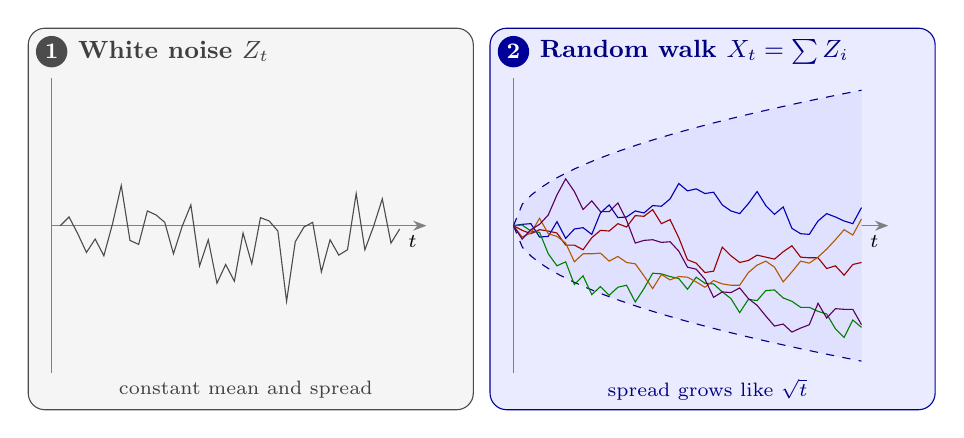
\begin{tikzpicture}[scale=0.85]
\foreach \px/\col/\num/\name/\eqn in {
 0/gray/1/{White noise $Z_t$}/{constant mean and spread},
 6.9/blue/2/{Random walk $X_t = \sum Z_i$}/{spread grows like $\sqrt t$}} {
 \begin{scope}[shift={(\px,0)}]
  \filldraw[fill=\col!8,draw=\col!60!black,rounded corners=6pt] (-0.35,-2.75) rectangle (6.3,2.95);
  \node[circle,fill=\col!60!black,text=white,inner sep=1.5pt,font=\footnotesize\bfseries] at (0,2.6) {\num};
  \node[anchor=west,font=\small\bfseries,text=\col!50!black] at (0.25,2.6) {\name};
  \draw[-Stealth,gray] (0,0) -- (5.6,0) node[below left,black,font=\scriptsize] {$t$};
  \draw[-,gray] (0,-2.2) -- (0,2.2);
  \node[font=\scriptsize,text=\col!50!black] at (2.9,-2.45) {\eqn};
  \ifnum\num=1
   \draw[-,gray!60!black] plot coordinates {(0.13,0.00) (0.26,0.13) (0.39,-0.12) (0.52,-0.40) (0.65,-0.20) (0.78,-0.45) (0.91,0.03) (1.04,0.60) (1.17,-0.22) (1.30,-0.28) (1.43,0.22) (1.56,0.16) (1.69,0.05) (1.82,-0.42) (1.95,-0.01) (2.08,0.31) (2.21,-0.60) (2.34,-0.21) (2.47,-0.86) (2.60,-0.58) (2.73,-0.83) (2.86,-0.11) (2.99,-0.57) (3.12,0.12) (3.25,0.07) (3.38,-0.08) (3.51,-1.13) (3.64,-0.24) (3.77,-0.02) (3.90,0.05) (4.03,-0.69) (4.16,-0.21) (4.29,-0.44) (4.42,-0.36) (4.55,0.48) (4.68,-0.36) (4.81,-0.01) (4.94,0.40) (5.07,-0.26) (5.20,-0.05)};
  \fi
  \ifnum\num=2
   \fill[blue!12] plot[domain=0:5.2,samples=40] (\x,{0.32*sqrt(\x/0.13)}) -- plot[domain=5.2:0,samples=40] (\x,{-0.32*sqrt(\x/0.13)}) -- cycle;
   \draw[-,dashed,blue!50!black] plot[domain=0:5.2,samples=40] (\x,{0.32*sqrt(\x/0.13)});
   \draw[-,dashed,blue!50!black] plot[domain=0:5.2,samples=40] (\x,{-0.32*sqrt(\x/0.13)});
   \draw[-,blue!70!black] plot coordinates {(0,0) (0.13,0.02) (0.26,0.03) (0.39,-0.17) (0.52,-0.16) (0.65,0.06) (0.78,-0.19) (0.91,-0.05) (1.04,-0.03) (1.17,-0.13) (1.30,0.19) (1.43,0.31) (1.56,0.12) (1.69,0.13) (1.82,0.22) (1.95,0.19) (2.08,0.30) (2.21,0.29) (2.34,0.40) (2.47,0.63) (2.60,0.52) (2.73,0.55) (2.86,0.48) (2.99,0.50) (3.12,0.31) (3.25,0.22) (3.38,0.18) (3.51,0.33) (3.64,0.51) (3.77,0.30) (3.90,0.17) (4.03,0.28) (4.16,-0.04) (4.29,-0.12) (4.42,-0.13) (4.55,0.07) (4.68,0.18) (4.81,0.13) (4.94,0.07) (5.07,0.03) (5.20,0.27)};
   \draw[-,red!60!black] plot coordinates {(0,0) (0.13,-0.07) (0.26,-0.12) (0.39,-0.06) (0.52,-0.08) (0.65,-0.11) (0.78,-0.29) (0.91,-0.29) (1.04,-0.36) (1.17,-0.18) (1.30,-0.07) (1.43,-0.08) (1.56,0.03) (1.69,-0.02) (1.82,0.15) (1.95,0.14) (2.08,0.24) (2.21,0.03) (2.34,0.09) (2.47,-0.18) (2.60,-0.51) (2.73,-0.56) (2.86,-0.70) (2.99,-0.68) (3.12,-0.32) (3.25,-0.45) (3.38,-0.55) (3.51,-0.52) (3.64,-0.44) (3.77,-0.47) (3.90,-0.50) (4.03,-0.39) (4.16,-0.30) (4.29,-0.47) (4.42,-0.48) (4.55,-0.48) (4.68,-0.64) (4.81,-0.60) (4.94,-0.74) (5.07,-0.58) (5.20,-0.55)};
   \draw[-,green!50!black] plot coordinates {(0,0) (0.13,0.01) (0.26,-0.08) (0.39,-0.10) (0.52,-0.42) (0.65,-0.60) (0.78,-0.54) (0.91,-0.88) (1.04,-0.75) (1.17,-1.03) (1.30,-0.91) (1.43,-1.04) (1.56,-0.92) (1.69,-0.89) (1.82,-1.14) (1.95,-0.94) (2.08,-0.71) (2.21,-0.72) (2.34,-0.76) (2.47,-0.79) (2.60,-0.95) (2.73,-0.77) (2.86,-0.86) (2.99,-0.87) (3.12,-0.99) (3.25,-1.09) (3.38,-1.30) (3.51,-1.10) (3.64,-1.12) (3.77,-0.97) (3.90,-0.96) (4.03,-1.08) (4.16,-1.13) (4.29,-1.22) (4.42,-1.22) (4.55,-1.28) (4.68,-1.32) (4.81,-1.54) (4.94,-1.67) (5.07,-1.41) (5.20,-1.52)};
   \draw[-,orange!70!black] plot coordinates {(0,0) (0.13,-0.17) (0.26,-0.11) (0.39,0.11) (0.52,-0.12) (0.65,-0.16) (0.78,-0.26) (0.91,-0.54) (1.04,-0.42) (1.17,-0.42) (1.30,-0.41) (1.43,-0.53) (1.56,-0.46) (1.69,-0.55) (1.82,-0.57) (1.95,-0.75) (2.08,-0.94) (2.21,-0.73) (2.34,-0.81) (2.47,-0.76) (2.60,-0.77) (2.73,-0.84) (2.86,-0.92) (2.99,-0.82) (3.12,-0.87) (3.25,-0.89) (3.38,-0.89) (3.51,-0.70) (3.64,-0.59) (3.77,-0.53) (3.90,-0.62) (4.03,-0.84) (4.16,-0.69) (4.29,-0.53) (4.42,-0.56) (4.55,-0.47) (4.68,-0.35) (4.81,-0.21) (4.94,-0.06) (5.07,-0.14) (5.20,0.10)};
   \draw[-,violet!70!black] plot coordinates {(0,0) (0.13,-0.20) (0.26,-0.06) (0.39,0.02) (0.52,0.16) (0.65,0.46) (0.78,0.70) (0.91,0.51) (1.04,0.24) (1.17,0.37) (1.30,0.21) (1.43,0.21) (1.56,0.34) (1.69,0.08) (1.82,-0.26) (1.95,-0.22) (2.08,-0.21) (2.21,-0.25) (2.34,-0.24) (2.47,-0.38) (2.60,-0.62) (2.73,-0.65) (2.86,-0.80) (2.99,-1.07) (3.12,-0.99) (3.25,-1.00) (3.38,-0.93) (3.51,-1.09) (3.64,-1.19) (3.77,-1.35) (3.90,-1.50) (4.03,-1.47) (4.16,-1.59) (4.29,-1.53) (4.42,-1.48) (4.55,-1.16) (4.68,-1.38) (4.81,-1.24) (4.94,-1.25) (5.07,-1.25) (5.20,-1.48)};
  \fi
 \end{scope}
}
\end{tikzpicture}
\caption{(1) A realisation of white noise. (2) Five realisations of a random walk with $\mu = 0$, started at $0$, with
the band $\pm2\sigma_Z\sqrt t$ (shaded) within which about $95\%$ of paths lie at each time. The walk is not stationary: its
spread keeps growing.}
\label{fig:random-walk}
\end{figure}

\begin{exa}\label{exa:drift}
A share price is modelled as a random walk with drift, $X_t = X_{t-1} + Z_t$, with $X_0 = 0$ measured from today's price and
daily changes $Z_t \sim N(0.5, 4)$, independent. Find the mean and variance of the price change over ten days, the
probability that it exceeds $10$, and the correlation between the changes over ten and twenty days.
\end{exa}

\begin{solution}
By Theorem~\ref{thm:random-walk}, $E(X_{10}) = 10(0.5) = 5$ and $\Var(X_{10}) = 10(4) = 40$, so $\operatorname{sd}(X_{10}) = 6.32$. As a sum of independent
normal variables, $X_{10}$ is normal, and
\[
P(X_{10} > 10) = P\Bigl(Z > \frac{10 - 5}{6.32}\Bigr) = P(Z > 0.79) = 0.215 .
\]
The correlation between $X_{10}$ and $X_{20}$ is $\sqrt{10/20} = 0.71$: half of the twenty-day change is the ten-day change, so the
two are strongly related. The drift adds $0.5$ a day on average, but after ten days its effect, $5$, is smaller than one
standard deviation of the noise, which is why the random walk is so hard to forecast.
\end{solution}

\subsection{Practice problems}
\begin{problem}\label{prob:ts-ma1-stationary}
Let $\{Z_t\}$ be white noise with mean $0$ and variance $\sigma_Z^2$, and $X_t = Z_t + 0.5Z_{t-1}$. Find $E(X_t)$, $\gamma(k)$ and $\rho(k)$, and show
that the process is stationary.
\end{problem}

\begin{solution}
$E(X_t) = 0$. $\gamma(0) = \Var(Z_t) + 0.25\Var(Z_{t-1}) = 1.25\sigma_Z^2$. For $k = 1$, $\Cov(Z_t + 0.5Z_{t-1}, Z_{t+1} + 0.5Z_t) = 0.5\Var(Z_t) = 0.5\sigma_Z^2$. For $|k| \ge 2$ the
two variables involve no common $Z$, so $\gamma(k) = 0$. None of this depends on $t$, so the process is stationary, with
$\rho(1) = 0.5/1.25 = 0.4$ and $\rho(k) = 0$ for $|k| \ge 2$.
\end{solution}

\begin{problem}\label{prob:ts-sign}
Let $Z$ be a single random variable with mean $0$ and variance $\sigma^2$, and $X_t = (-1)^tZ$. Is $\{X_t\}$ stationary? What do its
realisations look like?
\end{problem}

\begin{solution}
$E(X_t) = 0$ and $\Cov(X_t, X_{t+k}) = (-1)^{2t+k}\Var(Z) = (-1)^k\sigma^2$, which depends only on $k$. So it is stationary, with $\rho(k) = (-1)^k$. Each
realisation simply alternates between $Z$ and $-Z$: one random number decides the whole path. Stationarity
does not mean the series is random-looking, only that its moments do not change with time.
\end{solution}

\begin{problem}\label{prob:ts-rw-increment}
For a random walk with drift $\mu$ and variance $\sigma_Z^2$, show that $X_t - X_{t-k}$ has mean $k\mu$ and variance $k\sigma_Z^2$ for every $t$. Is $\{X_t - X_{t-k}\}$,
for fixed $k$, a stationary process?
\end{problem}

\begin{solution}
$X_t - X_{t-k} = Z_{t-k+1} + \dots + Z_t$, a sum of $k$ independent terms, so its mean is $k\mu$ and its variance $k\sigma_Z^2$, whatever $t$. As a moving sum
of white noise it is stationary: $\Cov(X_t - X_{t-k}, X_{t+j} - X_{t+j-k})$ is $\sigma_Z^2$ times the number of $Z$'s the two sums share, which is $\max(k - |j|, 0)$,
a function of $j$ alone.
\end{solution}

\begin{problem}\label{prob:ts-not-acf}
Let $\rho(\pm1) = 0.6$, $\rho(0) = 1$ and $\rho(k) = 0$ otherwise. The determinants $D_n = \det\mathbf{R}_n$ satisfy $D_n = D_{n-1} - 0.36D_{n-2}$, with $D_1 = 1$ and
$D_2 = 0.64$. Show that $D_3$ and $D_4$ are positive but $D_5$ is negative, and conclude.
\end{problem}

\begin{solution}
Expanding $\det\mathbf{R}_n$ along its first row gives the recursion, since $\mathbf{R}_n$ is tridiagonal. Then
$D_3 = 0.64 - 0.36 = 0.28$, $D_4 = 0.28 - 0.36(0.64) = 0.0496$ and $D_5 = 0.0496 - 0.36(0.28) = -0.0512 < 0$. So $\mathbf{R}_5$ is not non-negative definite, and the
function is not an ac.f., even though the $3 \times 3$ and $4 \times 4$ checks pass. Checking a few small matrices is not enough in
general; for this shape of function, the exact condition is $|\rho(1)| \le \frac12$, and $0.6$ exceeds it.
\end{solution}

\section{Moving Average (Ma)}\label{sec:ma}
Let $\{Z_t\}$ be a purely random process with mean $\mu = 0$ and variance $\sigma^2$. Then $\{X_t\}$ is a moving average process of order q written as
$$X_t = \beta_0Z_t + \beta_1Z_{t-1} + \beta_2Z_{t-2} + ............... + \beta_qZ_{t-q}$$
where $\{\beta_{j's}\}$ are constants. We normally assume $\beta_0 = 1$\\\\

We write MA(q) to denote Moving Average of order q.\\
$E(X_t) = 0$\hspace{0.2cm}   since \hspace{0.2cm}$E(\beta_0Z_t) + E(\beta_1Z_{t-2}) + ......+ E(\beta_qZ_{t-q}) = 0 + 0 + \cdots+ 0$\\
$var(X_t) = \sum\limits^2_Z\sum\limits^q_{j=0}\beta^2_j$\\

Since $Z_{t's}$ are independent
\begin{align*}
\varphi(k) &= Cov(X_t,X_{t+k})\\
           &= Cov(\beta_0Z_t + \beta_1Z_{t-1} +\cdots\cdots+ \beta_qZ_{t-q},\beta_0Z_{t+k} + \beta_1Z_{t+k-1} +\cdots\cdots+ \beta_qZ_{t+k-q})\\
\end{align*}           
\[\implies\hspace{0.6cm}\varphi(k) =
\begin{cases}
0, &k>q\\\\
\sigma^2_Z\sum\limits^{q-k}_{i=0}\beta_i\beta_{i+k}, &k = 0, 1, 2,\cdots\cdots, q\\\\
\varphi(-k),& k<0.\\
\end{cases} 
\]\\ 

 
\[\text{Since}\hspace{1cm} Cov(Z_s,Z_t) =
\begin{cases}
\sigma^2_Z, &s=t\\
0, &s\neq t\\
\end{cases}
\]\\

As $\varphi(k)$ does not depend on t and the mean is constant, the process is second order stationary for all values $\{\beta_i\}$.\\\\
ac.f of MA(q) is
\[ \rho(\mu) =
\begin{cases}
1, &k = 0\\\\
\dfrac{\sum\limits^{q-k}_{i=0}\beta_i\beta_{i+k}}{\sum\limits^q_{i=0}\beta^2_i}, &k = 1, \cdots\cdots, q\\\\
\rho(-k), &k<0
\end{cases}
\]\\

In particular the MA(1) with $\beta_0 = 1$ is $X_t = Z_t + \beta_1Z_{t-1}$. We have that
\[ \rho(k) = 
\begin{cases}
1, &k = 0\\
\dfrac{\beta_1}{1 + \beta^2_1}, &k = 1, 2,\cdots\cdots, q\\
0, & \text{otherwise}
\end{cases}
\]\\\\\\









\pagebreak
\section{Invertibility}\label{sec:invertibility}
This imposes restrictions on the $\{\beta_i\}$ to ensure that the process satisfies the invertibility conditions.\\

Consider the first order MA(1)
$$\text{A}: X_t = Z_t + \theta Z_{t-1}$$
$$\text{B}: X_t = Z_t + \frac{1}{\theta} Z_{t-1}$$
these functions have the same auto correlation function. Thus we can't classify many MA uniquely from a given auto correlation function.\\


We express A and B in terms of $X_t$ and $X_{t-1}$
$$\text{A}: Z_t = X_t - \theta X_{t-1} + \theta^2 X_{t-2}$$
$$\text{B}: Z_t = X_t - \frac{1}{\theta} X_{t-1} + \frac{1}{\theta^2} X_{t-2}$$
If $|\theta| < 1$ the process A converges while the series B diverges.\\
Thus, if $|\theta| < 1$ the model A is convertible while B is not.\\
The impression of the invertibility condition ensures that there is a unique process for a given auto correlation.\\
To compute the invertibility condition for MA. We express it by the use of the backward shift given by\\

$\beta^j X_t = X_{t-j},    \hspace{1cm}\forall j$\\

$\beta^2 X_t = X_{t-2}$, $\hspace{1cm}\beta X_t = X_{t-1}$\\

Thus $\hspace{0.2cm} X_t = \beta_0Z_t + \beta_1Z_{t-1} + \cdots\cdots+ \beta_qZ_{t-q}\hspace{0.2cm}$ can be written as
\begin{align*}
X_t &= (\beta_0 + \beta_1B + \beta_2B^2 + \cdots\cdots + \beta_qB^q)Z_t\\        
    &= \theta(B)Z_t\\
\end{align*}   

 
Where $\theta(B)$ is a polynomial of order q in B.\\
An MA(q) is invertible if the roots of the equation $\theta(B) = 0$\\
i.e $\hspace{0.2cm}\beta_0 + \beta_1B + \beta_2B^2 + .......... + \beta_qB_q = 0$ \hspace{0.2cm},\hspace{0.2cm} lie outside a unit circle.\\\\




\vspace{3cm}

EXAMPLE:\\
MA(1) , $\hspace{0.2cm} X_t = Z_t + \theta Z_{t-1}= (1 + \theta B)Z_t$ or $\theta(B) = 1 + \theta B$\\ 
The roots of $\theta (B) = 0$ are $B = \dfrac{-1}{\theta}$\hspace{0.2cm},\hspace{0.2cm}
the root is outside the unit circle provided $|\theta| < 1$.\\






\pagebreak


\section{Autoregressive Process}
Let $\{Z_t\}$ be a process with mean zero and variance $\sigma^2_Z$. Then $\{X_t\}$ is said to be an AR of order p or AR(p) if $X_t = \alpha_1 X_{t-1} + \alpha_2 X_{t-2} + \cdots\cdots + \alpha_p X_{t-p} + Z_t$\\



The first order process i.e AR(1) or $p = 1$\\
$X_t = \alpha X_{t-1} + Z_t$, $\hfill( X_{t-1} = \alpha X_{t-2} + Z_{t-1})$\\
or\\
$X_t = \alpha (\alpha X_{t-3} + Z_{t-1}) + Z_t$\\
$X_t = \alpha^2 (\alpha X_{t-3} + Z_{t-2}) + \alpha Z_{t-1} + Z_t$\\

so that $X_t$ is expressed in terms of $Z_t$ or an infinite order MA process provided $|\alpha| < 1$.
$$X_t = Z_t + \alpha Z_{t-1} + \alpha^2 Z_{t-2} + \alpha^3 Z_{t-3} +\cdots +\cdots$$
this is the duality between AR and MA process.\\\\



\begin{note}
$X_t = \alpha X_{t-1} + Z_t$ can be written as $(1 - \alpha B)X_t = Z_t$ using the backward shift operator. Therefore,
\begin{align*}
X_t &= \frac{Z_t}{1 - \alpha B}\\
    &= (1 + \alpha B + \alpha^2 B^2+ \alpha^3 B^3 + ............ +...)Z_t\\
    &= Z_t + \alpha Z_{t-1} + \alpha^2 Z_{t-2} + .................. \\
\end{align*}
Thus $E(X_t) = 0$ because $X_t$ is a purely random process and



\begin{align*}
var(X_t) &= (1 + \alpha^2 + \alpha^4 + .............)\sigma^2_Z\\
         &= \frac{\sigma^2_Z}{1 - \alpha^2}
\end{align*}
provided $|\alpha| < 1$\\\\




\vspace{4cm}

The acv.f is given by
\begin{align*}
\varphi(k) &= E(X_t,X_{t+k})\\
           &= E\Big[\Big(\sum\alpha^i Z_{t-i}\Big)\Big(\sum\alpha^i Z_{t+k-i}\Big)\Big]\\
           &= \sigma^2_Z \sum^{\infty}_{i=0} \alpha^i \alpha^{k+i}, \hspace{2cm} for \hspace{0.3cm} k\geq 0      
\end{align*}
which converges for $|\alpha| < 1$ to
\begin{align*}
\varphi(k) &= \frac{\alpha^k \sigma^2_Z}{1 - \alpha^2}\\
           &= \alpha^k \sigma^2_x\hspace{0.5cm},   \hspace{1.5cm} var(X_t) = \sigma^2_x = \frac{\sigma^2_Z}{1 - \alpha^k}
\end{align*}
for $\hspace{0.2cm} k < 0\hspace{0.3cm}$, $\hspace{0.3cm} \varphi(k) = \varphi(-k)$\\
$\varphi(k)$ does not depend on $t$, an AR(1) is second order stationary provided $|\alpha| < 1$. The ac.f is given by\\
$$\rho(k) = \alpha^k, \hspace{1cm} k = 0, \pm1, \pm2, \cdots\cdots$$\\





For $X_t = \alpha X_{t-1} + Z_t,  \hspace{1cm}(AR(1)) $, we can multiply this by $X_{t-k}$ to obtain\\
$$X_{t-k}X_t = \alpha X{t-k}\,\cdot \, X_{t-1} + X_{t-k}\,\cdot\, Z_t$$
taking the expectation, we have
$\hspace{0.3cm}\boxed{\varphi(-k) = \alpha \varphi(-k+1)}\hspace{0.3cm}$ on the assumption that $E(X_{t-k}\,\cdot\, Z_t) = 0$, for $k>0$.\\

Since $\varphi(-k) = \varphi(k)$ we have $\varphi(k) = \alpha \varphi(k-1)$ for $k > 0$.\\
Since $\varphi(0) = \sigma^2_X$, thus $\varphi(k) = \alpha^k \sigma^2_X$ for $k\geq0$,
thus 
$$\rho(k) = \frac{\varphi(k)}{\varphi(0)} = \frac{\alpha^k \sigma^2_X}{\sigma^2_X} = \alpha^k\hspace{0.2cm},\hspace{0.2cm} \text{for}\hspace{0.2cm} k\geq0.$$

Since, $|\rho(k)|<1$ we must have $|\alpha|<1$.\\
If $|\alpha|=1$, then $|\rho(k)|=1$,for all  k this is a degenerate case. Thus $|\alpha|<1$ for a proper, stationary time series.\\\\\\






\vspace{3cm}
\end{note}
\subsection{General Order Of an AR Process}
Let AR be expressed as an MA Process. Consider the equation
$$X_t = \alpha_1 X_{t-1} + \alpha_2 X_{t-2} + \cdots\cdots + \alpha_p X_{t-p} + Z_t, \hspace{1cm} AR(p)$$

$$\text{or}\hspace{0.5cm}(1 - \alpha_1 B - \alpha_2 B^2 --------- \alpha_p B^p)X_t = Z_t$$



\begin{align*}
\text{or}\hspace{0.5cm} X_t & = \frac{Z_t}{1 - \alpha_1 B - \alpha_2 B^2 --------- \alpha_p B^p}\\
X_t & = f(B)Z_t
\end{align*}

where
\begin{align*}
f(B) &= (1 - \alpha_1 B - \alpha_2 B^2 ----------\alpha_p B^p)^{-1}\\
     &= 1 + \beta_1 B + \beta_2 B^2 + \cdots\cdots
\end{align*}
the $\alpha_i$ and $\beta_i$ can be found.\\



Since $X_t$ is in terms of an MA, $E(X_t)=0$ and the variance is finite provided $\sum\limits^{\infty}_{i=0} \beta^2_i$ converge.\\

The acv.f is given by
$$\varphi(k)= \sigma^2_Z \,\sum^{\infty}_{i=0} \beta_i \beta_{i+k}\hspace{0.3cm},\hspace{0.3cm} \text{where}\hspace{0.3cm} \beta_0=1$$ the sufficient condition for this to converge , $\Sigma|\beta_i|$ converge\\




To find the ac.f, we assume as stationality we multiply $$X_t= \alpha_1 X_{t-1} + \alpha_2 X_{t-2} + \cdots\cdots+ \alpha_p X_{t-p}$$ by $X_{t-k}$ and take expectations and divide by $\sigma^2_X$. Assuming $var(X_t)$ is finite. We have
$$\rho(k)= \alpha_1 \rho(k-1) + \cdots\cdots + \alpha_p \rho(k-p)\hspace{0.3cm},\hspace{0.3cm} \forall k\geq0$$
This is called Yule Walker equations and this has a general solution
$$\rho(k)= A_1\pi^{|k|}_1 + A_2\pi^{|k|}_2 + \cdots\cdots+ A_p\pi^{|k|}_p$$
and the $\{\pi_i\}$ are the roots of the auxiliary equation.
$$Y^p - \alpha_1 Y^{p-1} - \alpha_2 Y^{p-2} -------- \alpha_p = 0$$
Then the $A_{i's}$ are chosen to satisfy the initial conditions depending on $\rho(0)=1$, i.e $\sum A_i=1$.\\
This first Yule Walker equations provide several routes to estimating the parameters of AR(p) model, by replacing the theoretical covariances with estimated values. Further restrictions on the $\{A_{i's}\}$ using $\rho(0)=1$ and $\rho(-k) = \rho(k)$.The general form of $\rho(k)$ tends to zero as $k\rightarrow \infty$ (increases) provided $|\pi_i|<1$, this is a necessary and sufficient condition for the process to be stationary.\\





An equivalent way to express stationality of AR(p) is to express the roots as $\phi(B) = 1 -\alpha_1 B -\alpha_2 B^2 --------- \alpha_p B^p=0$ must lie outside the unit circle.\\\\

\begin{exa}
Consider the AR(2) process $X_t=\alpha_1 X_{t-1}+\alpha_2 X_{t-2}+Z_t$ when $\pi_1$ and $\pi_2$ are the roots of the quadratic equation
$$Y^2- \alpha_1 Y- \alpha_2=0$$
We have $|\pi_i|<1$ if $\Bigg|\dfrac{\alpha_1 \pm\sqrt{\alpha^2_1 +4\alpha_2}}{2}\Bigg|<1$
the stationality region is in the triangular region such that $\alpha_1 +\alpha_2<1,\hspace{0.3cm} \alpha_1- \alpha_2>-1,\hspace{0.3cm} \alpha_2>-1$ the roots are real if $\alpha^2_1 +4\alpha_2>0$ and complex if $\alpha^2_1 + 4\alpha_2 <0$.\\
\end{exa}

When the roots are real $A_1$ and $A_2$ can be found as follows, since $\rho(0)=1$\\
from $\rho(k)= A_1\pi^{|k|}_1 +A_2\pi^{|k|}_2 +...............+ A_p\pi^{|k|}_p$


\begin{align*}
\rho(0) &= A_1\pi^{|0|}_1 + A_2\pi^{|0|}_2\\
         &= A_1 + A_2\\
         1&=A_1 + A_2
\end{align*}
from the Yule Walker equation\\
$\rho(k)=\alpha_1 \rho(k-1) +\alpha_2 \rho(k-2) + ..........+ \alpha_p \rho(k-p), \forall k\geq0$\\

we have\\
\begin{align*}
\rho(1) &=\alpha_1 \rho(1-1) + \alpha_2 \rho(1-2)\\
        &=\alpha_1 \rho(0) +\alpha_2 \rho(-1)\\
        &=\alpha_1 \rho(0) +\alpha_2 \rho(1)\\\\
 \implies \rho(1)       &=\alpha_1 +\alpha_2 \rho(1)\\\\
 \implies \rho(1) &=\frac{\alpha_1}{1-\alpha_2}\\
\end{align*}

$\rho(1)= A_1\pi_1 + A_2\pi_2$\\
But $1= A_1+A_2$ or $1-A_1=A_2$ \hspace{0.2cm},\hspace{0.2cm} Therefore
\begin{align*}
\rho(1) &= A_1\pi_1 +A_2\pi_2\\
        &= A_1\pi_1 +(1-A_1)\pi_2\\\\
\implies \frac{\alpha_1}{1-\alpha_2} &=A_1\pi_1 +(1-A_1)\pi_2 \\\\
\implies A_1 &= \frac{\Big[\dfrac{\alpha_1}{1-\alpha_2}-\pi_2\Big]}{\pi_1 -\pi_2}\\\\
\implies A_2 &= 1-A_1\\
             &= \frac{\pi_1 -\pi_2 -\Big[\dfrac{\alpha_1}{1-\alpha_2}-\pi_2\Big]}{\pi_1 -\pi_2}\\      
\end{align*}










\begin{exa}
Consider an AR(2)\hspace{0.2cm},\hspace{0.3cm} $X_t=X_{t-1}-\dfrac{1}{2}X_{t-2}+Z_t$. Is this process stationary and if so what is its ac.f.\\
\end{exa}


\begin{solution}
We find the roots of $\phi(B) =1-B+\frac{1}{2}B^2=0$.   The roots are $1\pm2$,the modules of both roots exceed one, therefore there are outside the unit circle. Thus the process is stationary.\\ To find the ac.f, we use the first Yule- Walker equation 
$$\rho(1)= \rho(0)-\frac{1}{2}\rho(-1)$$ Giving $\hspace{0.2cm}\rho(1)=\dfrac{2}{3}$\\
\end{solution}

for $k\geq2$,\\ $\rho(k) =\rho(k-1)-\dfrac{1}{2}\rho(k-2)$ and $\rho(2), \rho(3)$ can be found by successive substitution.\\\\\\






\section{Mixed Arma Models}
The MA and AR models can be combined to obtain an ARMA model.  A mixed ARMA with p AR terms and q MA terms is an ARMA process of order $(p,q)$
$$X_t=\alpha_1 X_{t-1}+\alpha_2 X_{t-2}+\cdots\cdots+\alpha_{p} X_{t-p}+Z_t+\beta_1 Z_{t-1}+\cdots\cdots+\beta_q Z_{t-q}$$ or\\
$\phi(B) X_t=\theta(B) Z_t $ where $\phi(B)$ and $\theta(B)$ are polynomials of order p and q respectively and
$$\phi(B)= 1-\alpha_1 B-\alpha_2 B^2- ------\alpha_p B^p$$
$$\theta(B)=1+\beta_1 B+\beta_2B^2 +.........+\beta_q B^q$$
For AR the values of $\{\alpha_i \}$ which makes the process stationary are such that the roots of $\phi(B) =0$ lie outside the unit circle.\\
Similarly for the MA process, the values of $\{\beta_i \}$ which make the process stationary are such that the roots of $\theta(B) =0$ lie outside the unit circle.\\
ARMA process are important in that a stationary time series may be described by an ARMA model involving few parameters than the pure MA or AR by itself.\\It is useful to express ARMA as pure MA process in the form $X_t=\psi(B) Z_t$, where $\psi(B) =\sum\psi_i \beta^i$. $\psi(B)$ is an MA operator and maybe of finite or infinite order.\\

From $\phi(B) X_t=\theta(B) Z_t$\hspace{0.2cm} we have \hspace{0.2cm}$\psi(B) =\dfrac{\theta(B)}{\phi(B)}$\hspace{0.2cm} and\hspace{0.2cm} $\pi(B) X_t=Z_t$\hspace{0.2cm} where\hspace{0.2cm} $\pi(B) =\dfrac{\phi(B)}{\theta(B)}$\\

That $\pi(B) =1- \sum\pi_i B^i $, since $X_t=\sum\limits^{\infty}_{i=0} \pi_i X_{t-i}+Z_t$\\


Thus from $X_t=\psi(B) Z_t$ and $\pi(B) X_t=Z_t$, we have $\psi(B)\,\cdot\,\pi(B) =1$
$$\implies\hspace{1cm}\frac{\theta(B)}{\phi(B)}\,\cdot\,\frac{\phi(B)}{\theta(B)}=1$$
the $\psi$ weight and $\pi$ weight maybe computed by equating the process of B in the equation $\psi(B) \phi(B) =\theta(B)$.\\\\








\begin{exa}
Find the $\psi$ and $\pi$ weights for this ARMA(1,1) given by $$X_t =0.5X_{t-1}+Z_t-0.3Z_{t-1}$$
Here\\ $\phi(B) =1-0.5B.........(1)$\\
\end{exa}

$\phi(B)X_t=(1-0.5B)X_t=X_t-0.5X_t$\\

$\theta(B) =1-0.3............(2)$\\ 

$\phi(B) =0$ and $\theta(B) =0$ have roots outside the unit circle, so the process is stationary and invertible.\\\\

(1)  $\phi(B) =1-0.5B=0$\\

$\implies B=\dfrac{1}{0.5}=2$\\

$\psi(B)=\dfrac{\theta(B)}{\phi(B)}=\dfrac{1-0.3B}{1-0.5B}$\\

$\psi(B) =(1-0.3B)(1-0.5B)^{-1}$\\

$\psi(B)=(1-0.3B)(1+0.5B+ 0.5^2B^2 +0.5^3B^3+\cdots\cdots)$\\

$\implies \psi(B)=1+0.2B+0.1B^2+0.005B^3+\cdots\cdots$\\ 

Hence $\psi_i = 0.2\times0.5^{i-1}$ for\hspace{0.3cm}$i=1,2,3\cdots\cdots\cdots$\\\\ 

Similarly show that(2) $\pi_i =0.2\times 0.3^{i-1}$ for $i= 1,2,\cdots\cdots$\\






\pagebreak

\section{Integrated Arma}\label{sec:integrated}
When a process is non- stationary it is necessary to remove non-stationary sources of variation. In the process
 $$X_t + \alpha_1 X_{t-1} + \alpha_2 X_{t-2} + \cdots\cdots + \alpha_p X_{t-p} + Z_t + \beta_1 Z_{t-1} + \cdots\cdots + \beta_q Z_{t-q}$$
$X_t$ is replaced by $\nabla^d X_t$ then the model is capable of describing a certain type of non-stationary series. This model is called an integrated model, written as $W_t= \nabla^d X_t=(1 - B)^d X_t$ then the ARMA process is of the form
 $$W_t= \alpha_1 W_{t-1} +\alpha_2 W_{t-2} +\cdots\cdots+\alpha_p W_{t-p} +Z_t +\beta_1 Z_{t-1} +\cdots\cdots+\beta_q Z_{t-q}$$
 
or\\ $\phi(B) W_t =\theta(B) Z_t$\\or \\ $\phi(B) (1-B)^dX_t=\theta(B) Z_t$\\

Thus we have an ARMA of order $(p,q)$ for $W_t$. While the equation $$\phi(B) (1-B)^dX_t =\theta(B) Z_t$$ describes    the $d^{th}$ difference of $X_t$ it is an ARIMA process of order $(p,d,q)$. The $X_t$ model is non-stationary as the AR operator $\phi(B) (1-B)^d$ has d roots outside the unit circle. In particular the value of $d$ is 1.
 \begin{align*}
 \nabla^2 X_t &=\nabla (X_t-X_{t-1})\\
                        &=(X_t-X_{t-1})-(X_{t-1}-X_{t-2})\\
                        &=X_t-2X_{t-1}+X_{t-2}\\\\\
 \end{align*}
 
 
 
 
 










\pagebreak 
\section{Forecasting}
 Let $X_1,X_2,..............,X_n$ be an observed time series. The problem is to estimate further values $X_{t+k}$, $\hspace{0.2cm} k $is called lead time. The forecast $X_{n+k}$ at time $n$ at $k$ steps ahead can be denoted by $\widehat{x}(n,k)$. Various methods for forecasting exist. No single method is universally available.\\ Forecasting is of the form of extrapolation condition of a characteristic of a time series.\\
 
 
 
 Forecasting Methods:  Are broadly based on
 \begin{enumerate}
 \item Subjective\\-judgment\\-intuition\\-business knowledge\\or any other relevant information.
 \item Univariate\\based on a model fitted only the passed observation of $\{X_t\}$ so that $\widehat{x}(n,k)$ depends only on $X_t,X_t,........,X_n$
 \item Multivariate\\Used for non-seasonal time series showing no trends. For time series with trends or seasonal patterns these need to be removed to produce stationarity.\\
 \end{enumerate}
 
 Suppose $X_1,X_2,.......,X_n$ is a non-seasonal time series with no trend. We take $X_{n+1}$ as a waited a sum of passed observations
 $$\widehat{x}(n,1)= C_0X_n+C_1X_{n-1}+C_2X_{n-2}+\cdots\cdots$$
 then $\{C_i\}$ are the weights (Geometric weights) are used so that\\ $C_i=\alpha (1-\alpha )^i, \hspace{0.5cm}i=1,2,....$ where $\alpha$ is such that $0<\alpha <1.$\\\\
 The $\hspace{0.3cm}\widehat{x}(n,1)=C_0X_n+C_1X_{n-1}+C_2X_{n-2}+\cdots\cdots$\\\\
becomes $\hspace{0.3cm}\widehat{x}(n,1)=\alpha X_n+\alpha (1-\alpha )X_{n-1}+\alpha (1-\alpha )^2X_{n-2}+\cdots\cdots\cdots$\\or

$$\widehat{x}(n,1)=\alpha X_n+(1-\alpha )\Big[\alpha X_{n-1}+\alpha (1-\alpha )X_{n-2}+\alpha (1-\alpha )^2X_{n-3}+\cdots\cdots\Big]$$ Therefore\hspace{0.3cm} $\widehat{x}(n,1)=\alpha X_n+(1-\alpha )\widehat{x}(n-1,1)$.\\
 
 
If $\widehat{x}(1,1)=X_1$, the equation can be used recursively to compute forecasting, this is called exponential smoothing.\\

We can also write
\begin{align*}
\widehat{x}(n,1) &=\alpha X_n+(1-\alpha )\widehat{x}(n-1,1)\\
             &=\alpha \Big[X_n-\widehat{x}(n-1,1)\Big] +\widehat{x}(n-1,1)\\
             &=\alpha e_n +\widehat{x}(n-1,1)
\end{align*} 
where $e$ is the prediction error at time n. The values of $\alpha$ depend on the time series properties, usually the values of $\alpha$ are taken $0.1\leq \alpha \leq0.3$.\\\\









\subsection{The Partial Autocorrelation Function}

The autocorrelation function alone cannot identify an autoregressive model. For
an AR$(1)$ process the correlation between $X_t$ and $X_{t+2}$ is
$\rho(2)=\phi^{2}$, which is not zero --- but none of it is direct. It is
entirely inherited through $X_{t+1}$. The partial autocorrelation is what
removes that inheritance.

\begin{defn}
The \emph{partial autocorrelation} at lag $k$, written $\phi_{kk}$, is the
correlation between $X_t$ and $X_{t+k}$ after removing the linear effect of the
intervening values $X_{t+1},\dots,X_{t+k-1}$:
$$\phi_{kk} = \Corr\left(X_t,\ X_{t+k} \;\middle|\; X_{t+1},\dots,X_{t+k-1}\right).$$
Equivalently, $\phi_{kk}$ is the coefficient of $X_{t-k}$ in the best linear
predictor of $X_t$ from the previous $k$ values.
\end{defn}

\begin{result}[Yule--Walker]
The partial autocorrelations solve
$$\rho(j) = \sum_{i=1}^{k}\phi_{ki}\,\rho(j-i),\qquad j=1,\dots,k,$$
and $\phi_{kk}$ is the last coefficient of that system. In matrix form, with
$R_k$ the $k\times k$ matrix of $\rho(i-j)$,
$$R_k\,\boldsymbol{\phi}_k = \boldsymbol{\rho}_k .$$
\end{result}

\begin{exa}
Compute $\phi_{11}$ and $\phi_{22}$ for a general stationary process.
\end{exa}

\begin{solution}
At $k=1$ the system is $\rho(1) = \phi_{11}$, so
$$\phi_{11} = \rho(1).$$
At $k=2$,
$$\rho(1) = \phi_{21} + \phi_{22}\rho(1),\qquad
\rho(2) = \phi_{21}\rho(1) + \phi_{22}.$$
Eliminating $\phi_{21}$,
$$\phi_{22} = \frac{\rho(2)-\rho(1)^{2}}{1-\rho(1)^{2}} .$$

For an AR$(1)$ process $\rho(k)=\phi^{k}$, so
$$\phi_{22} = \frac{\phi^{2}-\phi^{2}}{1-\phi^{2}} = 0 ,$$
exactly as the definition promises: once $X_{t+1}$ is accounted for, nothing
direct connects $X_t$ to $X_{t+2}$.
\end{solution}

\begin{result}[Identification]
The two functions cut off for opposite models, and this is what makes them
usable together:
$$\begin{array}{lll}
\text{Model} & \text{ACF} & \text{PACF}\\ \hline
\text{AR}(p) & \text{tails off} & \text{cuts off after lag } p\\
\text{MA}(q) & \text{cuts off after lag } q & \text{tails off}\\
\text{ARMA}(p,q) & \text{tails off} & \text{tails off}
\end{array}$$
\end{result}

\begin{note}
The duality is not a coincidence. An AR$(p)$ process is a finite regression on
its own past, so beyond lag $p$ there is no direct effect left to find and the
PACF is zero. An MA$(q)$ process is a finite sum of $q+1$ shocks, so beyond lag
$q$ the two windows share no shock at all and the ACF is zero. Each model is
finite in one representation and infinite in the other --- which is the
invertibility discussion of the previous section seen from the other side.

In practice both functions are estimated from data and neither cuts off exactly.
The usual rule is to treat a sample value as zero when it lies within
$\pm 1.96/\sqrt{n}$, since under the null that the true value is zero the sample
autocorrelation is approximately $N(0,1/n)$. With $n=100$ that band is about
$\pm0.2$, which is wide --- identification is a judgement, not a calculation,
and the reason Box--Jenkins insists on the verification step.
\end{note}

\begin{remark}
When both functions tail off, the process is ARMA and the orders cannot be read
off directly. The practical route is then to fit several candidate models and
compare them by an information criterion, penalising parameters:
$$\text{AIC} = -2\log L + 2r,\qquad \text{BIC} = -2\log L + r\log n ,$$
where $r$ is the number of estimated parameters. BIC penalises more heavily and
tends to choose the smaller model, which for forecasting is usually the safer
error to make.
\end{remark}


\section{Estimation Of Models}
To effectively use the model for forecasting the parameters of the model ought to be estimated\\


\subsection{Fitting an AR Model}
-what is the order of the process\\
-how can we estimate the parameters of the process\\


Suppose we have an AR(p) with mean $\mu$ given by
$$X_t-\mu =\alpha_1 (X_{t-1}-\mu)+\alpha_2 (X_{t-2}-\mu)+\cdots\cdots+\alpha_p (X_{t-p}-\mu)+Z_t$$


If $X_1,X_2,\cdots\cdots,X_n$ are the observations of a time series. The parameter i.e $\alpha_1 ,\alpha_2 ,\cdots\cdots,\alpha_p$ can be estimated by least square, by minimizing\\
$$S=\sum^{n}_{t=p+1}\Big[X_t-\mu -\alpha_1 (X_{t-1}-\mu )-\alpha_2 (X_{t-2}-\mu )-\,\cdots\cdots\,-\alpha_p (X_{t-p}-\mu)\Big]^2$$
with respect to $\mu ,\alpha_1 ,\alpha_2 ,..........., \alpha_p$.\\\\



\subsection{Fitting an MA Process}
Finding an MA process is more complex than the AR because the least squares method cannot be applied to the ARMA and the ARIMA.\\



\subsection{Box-Jenkins Seasonal (SARIMA) Model}
In practice main time series contain a seasonal periodic component which repeats every 's' observations. e.g with monthly observations $s=12$. $X_t$ depends on terms such that $X_{t-12}$ and perhaps $X_{t-24}$. As well as $X_{t-1},X_{t-2},\cdots\cdots$\\\\


Box-Jenkins have generalized the ARIMA model to deal with seasonality and find the general multiplicative ARIMA model (SARIMA)as
$$\phi_p(B) \Phi_P(B^s) W_t=\theta_q(B) \Theta_Q(B^s)Z_t$$
where $\hspace{0.3cm} W_t=\nabla^d\, \nabla^D_s X_t$, B denotes the backward shift operator, $\,\phi_p \,,\,\Phi_P ,\,\theta_q \,\text{and} \hspace{0.2cm}\Theta_Q$ are polynomials of order p,P,q,Q respectively. $Z_t$ denotes a purely random process.\\
If $P=1$ the term $\Phi_p(B^s)$ will be $(1- \text{constant}\, XB^s)$ which means that $W_t$ will depend on $W_{t-s}$ since $B^s\,W_t=W_{t-s}$. The variables $\{W_t\}$ are formed from the original series $\{X_t\}$ not only by simple difference to remove trend but also by seasonal difference to remove seasonality.\\

If $d=D=1$ and $s=12$
\begin{align*}
W_t &=\bigtriangledown \bigtriangledown_{12} X_t\\
    &=\bigtriangledown_{12} X_t-\bigtriangledown_{12} X_{t-1}\\
    &=(X_t-X_{t-12})-(X_{t-1}-X_{t-13})\\
\end{align*}


The model equation $\,\phi_p(B) \Phi_P(B^s) W_t=\theta_q(B) \Theta_Q(B^s) Z_t\,$ and $\,W_t=\nabla^d \,\nabla^D_s X_t$ is said to be a SARIMA model of order $\,(p,d,q)\times(P,D,Q)_s$.\\\\



\begin{exa}
Consider the SARIMA $(1,0,0)\times(0,1,1)_{12}$\\
\end{exa}

So we note that $s=12$ then the model\\
$\phi_p(B) \Phi_P(B^s) W_t=\theta_q(B) \Theta_Q(B^s) Z_t$ and $W_t=\nabla^d\, \nabla^D X_t$ can be written as\\\\ $(1-\alpha B)W_t=(1+\theta B^{12})$ where $W_t=\nabla_{12} X_t$\\\\we find $X_t=X_{t-12}+\alpha (X_{t-1}-X_{t-13})+Z_t+\theta Z_{t-12}$ so that $X_t$ depends on $X_{t-1},X_{t-12},X_{t-13}$ as the innovation time.\\





\pagebreak

\subsection{Forecasting: (Box-Jenkins Procedure)}
The main stages of the the Box-Jenkins procedure,
\begin{enumerate}
\item Identification: examining the data to identify a model
\item Estimation: Estimating parameters of the model
\item Diagnostic checking: examining residuals from the the fitted model to see if the model is adequate
\item Consideration of an alternative model. This is done when the first model appears to be inadequate.\\
\end{enumerate}






\subsection{Computation of Forecast}
Use of difference equations, if the model equation is known then $\widehat{x}(n,1)$ can be obtained from the model equation by replacing,\\- future values of $Z$ by zero.\\- future values of $X$ by there conditional expectation.\\- past values of $X$ and $Z$ by their observed values.\\






\begin{exa}
Consider the SARIMA $(0,0,1)\times(1,1,0)_{12}$ used where
$$X_t=X_{t-12}-\alpha(X_{t-1}-X_{t-13})+Z_t+\theta Z_{t-12}$$
\end{exa}

$$\widehat{x}(n,1)=X_{n-11}-\alpha (X_n-X_{n-12})+\theta Z_{n-11}$$

and

\begin{align*}
\widehat{x}(n,2) &=X_{n-10}-\alpha (X_{t+1}-X_{n-11})+\theta Z_{n-10}\\
             &=X_{n-10}+\alpha (\widehat{x}(n,1)-X_{n-11})+\theta Z_{n-10}
\end{align*} 
forecasting further in the future can be calculated recursively when $X_{n+1}$ is known.


\begin{align*}
\widehat{x}(n+1,1) &=X_{n-10}+\alpha (X_{n+1}-X_{n-11})+\theta Z_{n-10}\\
               &=\widehat{x}(n,2)+\alpha (X_{n+1}-\widehat{x}(n,1))+\theta Z_{n-10}\\
               &=\widehat{x}(n,2)+\alpha Z_{n+1}
\end{align*}

\pagebreak


\section{The Frequency Domain}\label{sec:frequency}

Everything so far has described a series by how each value relates to the ones
before it. The frequency domain describes the same series by which
\emph{cycles} it is made of. Neither view adds information the other lacks ---
they are Fourier transforms of one another --- but each makes different things
obvious, and periodicity is far easier to see as a peak than as a pattern in the
autocorrelations.

\subsection{The Spectral Density}

\begin{defn}
For a stationary process with autocovariance $\gamma(\tau)$ satisfying
$\sum_{\tau}\left|\gamma(\tau)\right|<\infty$, the \emph{spectral density} is
$$f(\omega) = \frac{1}{2\pi}\sum_{\tau=-\infty}^{\infty}\gamma(\tau)\,e^{-i\omega\tau},
\qquad -\pi \leq \omega \leq \pi .$$
\end{defn}

\begin{result}
The autocovariance is recovered by inversion,
$$\gamma(\tau) = \int_{-\pi}^{\pi} f(\omega)\,e^{i\omega\tau}\,d\omega ,$$
and in particular
$$\gamma(0) = \Var(X_t) = \int_{-\pi}^{\pi} f(\omega)\,d\omega .$$
\end{result}

\begin{note}
The last line is the interpretation. The total variance of the series is
distributed across frequencies, and $f(\omega)\,d\omega$ is the share
contributed by cycles near frequency $\omega$. A peak in the spectrum is a
frequency band doing a disproportionate amount of the work --- which is exactly
what a seasonal effect looks like, and it is visible at a glance where the
autocorrelation function would show only a slow ripple.
\end{note}

\begin{exa}
Find the spectral density of white noise, and of the AR$(1)$ process
$X_t = \phi X_{t-1} + \varepsilon_t$.
\end{exa}

\begin{solution}
\subhead{White noise}
Here $\gamma(0)=\sigma^{2}$ and $\gamma(\tau)=0$ otherwise, so only one term
survives:
$$f(\omega) = \frac{\sigma^{2}}{2\pi},$$
constant in $\omega$. Every frequency contributes equally --- which is what the
name means, by analogy with white light.

\subhead{AR(1)}
For the AR$(1)$, $\gamma(\tau) = \dfrac{\sigma^{2}\phi^{|\tau|}}{1-\phi^{2}}$.
Summing two geometric series,
$$f(\omega) = \frac{\sigma^{2}}{2\pi}\cdot\frac{1}{\left|1-\phi e^{-i\omega}\right|^{2}}
= \frac{\sigma^{2}}{2\pi\left(1 - 2\phi\cos\omega + \phi^{2}\right)} .$$
For $\phi>0$ this is largest at $\omega=0$: the series is dominated by slow
movement, which is what positive autocorrelation means. For $\phi<0$ the peak
moves to $\omega=\pi$, the fastest representable oscillation --- alternation
from one observation to the next.
\end{solution}

\subsection{The Periodogram}

\begin{defn}
Given data $x_1,\dots,x_n$, the \emph{periodogram} at the Fourier frequencies
$\omega_j = 2\pi j/n$ is
$$I(\omega_j) = \frac{1}{2\pi n}\left|\sum_{t=1}^{n} x_t e^{-i\omega_j t}\right|^{2}.$$
\end{defn}

\begin{remark}
The periodogram is the natural estimate of the spectral density and it is a bad
one. It is asymptotically unbiased, but its variance does \emph{not} fall as $n$
grows: at each frequency $I(\omega_j)$ is approximately
$f(\omega_j)\chi^{2}_{2}/2$, whose variance is $f(\omega_j)^{2}$ however long the
series. Lengthening the record adds more frequencies rather than improving any
one of them.

The cure is smoothing --- averaging the periodogram over a window of
neighbouring frequencies. Averaging $m$ approximately independent ordinates cuts
the variance by a factor $m$ at the cost of blurring detail across the window,
which is the usual bias-variance trade and is chosen by how sharp the features
of interest are expected to be.
\end{remark}

\begin{note}
This is worth stating plainly because it is counter-intuitive: an estimator can
be consistent for the whole function in an integrated sense while being
inconsistent at every single point. The periodogram is the standard example, and
it is why raw periodograms look so ragged.
\end{note}

\section{State Space Models And The Kalman Filter}

An ARMA model describes a series directly. A state space model instead supposes
an unobserved process driving it, and the observations are a noisy view of that
process. The framework is more general --- every ARMA model can be written in
state space form --- and it handles missing data and time-varying parameters,
which ARMA cannot.

\subsection{The Linear Model}

\begin{defn}
A \emph{linear state space model} consists of two equations:
$$\textbf{x}_t = F\,\textbf{x}_{t-1} + \textbf{w}_t \qquad\text{(state equation)},$$
$$\textbf{y}_t = H\,\textbf{x}_t + \textbf{v}_t \qquad\text{(observation equation)},$$
where $\textbf{x}_t$ is the unobserved state, $\textbf{y}_t$ the observation, and
$\textbf{w}_t$, $\textbf{v}_t$ independent white noise with covariance matrices
$Q$ and $R$.
\end{defn}

\begin{note}
The state equation says the system evolves by its own dynamics; the observation
equation says we see it imperfectly. Separating the two is the whole idea. A
random walk observed with error --- $x_t = x_{t-1}+w_t$, $y_t = x_t+v_t$ --- is
the simplest non-trivial case, and it already cannot be written as an ARMA model
without first working out what its observable autocorrelation structure is.
\end{note}

\subsection{The Kalman Filter}

\begin{result}
Write $\widehat{\textbf{x}}_{t\mid s}$ for the expectation of $\textbf{x}_t$
given observations up to time $s$, and $P_{t\mid s}$ for its error covariance.
The Kalman filter alternates two steps.

\subhead{Predict}
$$\widehat{\textbf{x}}_{t\mid t-1} = F\,\widehat{\textbf{x}}_{t-1\mid t-1},
\qquad P_{t\mid t-1} = F\,P_{t-1\mid t-1}F^{t} + Q .$$

\subhead{Update}
With the \emph{innovation} $e_t = \textbf{y}_t - H\widehat{\textbf{x}}_{t\mid t-1}$
and the Kalman gain
$$K_t = P_{t\mid t-1}H^{t}\left(H P_{t\mid t-1}H^{t} + R\right)^{-1},$$
$$\widehat{\textbf{x}}_{t\mid t} = \widehat{\textbf{x}}_{t\mid t-1} + K_t e_t,
\qquad P_{t\mid t} = \left(I - K_tH\right)P_{t\mid t-1} .$$
\end{result}

\begin{remark}
Read the update as a weighted compromise. The innovation $e_t$ is the part of
the new observation the model did not anticipate, and the gain $K_t$ decides how
much of it to believe. If the observation noise $R$ is large the gain is small
and the filter trusts its own prediction; if the state noise $Q$ is large the
prediction is uncertain, the gain is near one, and the filter follows the data.
Everything the filter does is that trade, applied recursively.

The recursion is what makes it usable. Each step needs only the previous
estimate and the current observation, not the whole history, so the cost per
observation is constant and the filter runs in real time. That is why it is used
in navigation and tracking as much as in statistics.
\end{remark}

\begin{note}
The filter is optimal in two distinct senses that are worth keeping apart. If the
noise is Gaussian, $\widehat{\textbf{x}}_{t\mid t}$ is the conditional
expectation and therefore the best estimator of any kind. Without normality it
is still the best \emph{linear} estimator --- the same distinction as between
conditional expectation and linear regression.
\end{note}

\section{Nonlinear Models: ARCH And Volatility}

Every model so far has assumed constant variance. Financial series violate this
plainly: quiet periods and turbulent periods cluster, so the variance is itself
serially dependent even when the series is uncorrelated. ARCH models that
directly.

\begin{defn}
A process follows an \emph{ARCH}$(p)$ model if
$$X_t = \sigma_t\,\varepsilon_t,\qquad
\sigma_t^{2} = \alpha_0 + \sum_{i=1}^{p}\alpha_i X_{t-i}^{2},$$
where $\varepsilon_t$ is independent white noise with unit variance,
$\alpha_0>0$ and $\alpha_i\geq0$. The \emph{GARCH}$(p,q)$ extension adds lagged
variances,
$$\sigma_t^{2} = \alpha_0 + \sum_{i=1}^{p}\alpha_i X_{t-i}^{2}
+ \sum_{j=1}^{q}\beta_j \sigma_{t-j}^{2}.$$
\end{defn}

\begin{result}
For the ARCH$(1)$ model with $0\leq\alpha_1<1$:
$$E(X_t) = 0,\qquad \Var(X_t) = \frac{\alpha_0}{1-\alpha_1},
\qquad \Corr\left(X_t,\,X_{t+\tau}\right) = 0 \ \text{ for } \tau\neq0,$$
but $X_t^{2}$ is autocorrelated, following an AR$(1)$ in the squares.
\end{result}

\begin{proof}
Conditioning on the past, $E\left(X_t \mid \mathcal{F}_{t-1}\right)
= \sigma_t E(\varepsilon_t) = 0$, so $E(X_t)=0$ by the tower property and
$X_t$ is uncorrelated with anything earlier --- which gives the zero
autocorrelation.

For the variance, $E\left(X_t^{2}\right) = E\left(\sigma_t^{2}\right)
= \alpha_0 + \alpha_1E\left(X_{t-1}^{2}\right)$. Stationarity makes both
expectations equal, so $E\left(X_t^{2}\right)(1-\alpha_1) = \alpha_0$, giving the
stated variance and requiring $\alpha_1<1$ for it to be finite and positive.

Writing $\eta_t = X_t^{2}-\sigma_t^{2}$, which has mean zero, the definition
rearranges to
$$X_t^{2} = \alpha_0 + \alpha_1 X_{t-1}^{2} + \eta_t ,$$
an AR$(1)$ for the squared series.
\end{proof}

\begin{remark}
The last line is the whole point. The series itself is uncorrelated --- it passes
every test built on the autocorrelation function --- while its squares are
strongly correlated. A series can therefore be unpredictable in level and
entirely predictable in volatility, which is what makes returns look random
while their risk does not.

This is also the practical diagnostic: plot the ACF of the squared residuals
after fitting an ARMA model. If it is flat the constant-variance assumption
stands; if it decays slowly, an ARCH or GARCH term is needed. Nothing in the
ordinary residual ACF would have revealed it.
\end{remark}

\section{Practice Problems}

\begin{problem}
Show that the MA$(1)$ process $X_t = \varepsilon_t + \theta\varepsilon_{t-1}$ has
$\rho(1) = \theta/(1+\theta^{2})$ and $\rho(\tau)=0$ for $\tau\geq2$. Deduce the
largest value $\left|\rho(1)\right|$ can take.
\end{problem}
\begin{solution}
With $\Var(\varepsilon)=\sigma^{2}$,
$$\gamma(0) = \left(1+\theta^{2}\right)\sigma^{2},\qquad
\gamma(1) = \theta\sigma^{2},\qquad \gamma(\tau)=0 \ (\tau\geq2),$$
the last because $X_t$ and $X_{t+\tau}$ then share no shock. Dividing,
$$\rho(1) = \frac{\theta}{1+\theta^{2}},\qquad \rho(\tau)=0 \ (\tau\geq2).$$
Differentiating, $\rho(1)$ is extremised at $\theta=\pm1$, giving
$$\left|\rho(1)\right| \leq \tfrac12 .$$
So a sample first autocorrelation beyond $0.5$ in magnitude rules out an MA$(1)$
outright, whatever $\theta$ is chosen --- a genuine identification constraint,
not merely a guideline.

Note also that $\theta$ and $1/\theta$ give the same $\rho(1)$: the
autocorrelations do not determine the model, which is why invertibility is
imposed to pick the root inside the unit circle.
\end{solution}

\begin{problem}
An AR$(2)$ process is $X_t = 0.5X_{t-1} + 0.3X_{t-2} + \varepsilon_t$. Determine
whether it is stationary, and find $\rho(1)$ and $\rho(2)$.
\end{problem}
\begin{solution}
Stationarity requires the roots of the characteristic equation
$1 - 0.5z - 0.3z^{2} = 0$ to lie outside the unit circle. Solving,
$$z = \frac{0.5 \pm \sqrt{0.25 + 1.2}}{-0.6}
= \frac{0.5 \pm 1.204}{-0.6},$$
giving $z \approx -2.84$ and $z \approx 1.17$. Both exceed one in modulus, so the
process is stationary.

The Yule--Walker equations give
$$\rho(1) = \frac{\phi_1}{1-\phi_2} = \frac{0.5}{0.7} \approx 0.714 ,$$
$$\rho(2) = \phi_1\rho(1) + \phi_2 = 0.5(0.714) + 0.3 \approx 0.657 .$$
The slow decay is characteristic of an AR process: the ACF tails off rather than
cutting, and it is the PACF that would cut off after lag two.
\end{solution}

\begin{problem}
A series shows a clear upward trend and yearly seasonality in monthly data.
Describe the differencing needed before an ARMA model is fitted, and say what
model class results.
\end{problem}
\begin{solution}
A trend is removed by first differencing, $\nabla X_t = X_t - X_{t-1}$. Yearly
seasonality in monthly data is removed by seasonal differencing at lag twelve,
$\nabla_{12}X_t = X_t - X_{t-12}$. Applying both,
$$\nabla\nabla_{12}X_t = \left(X_t - X_{t-1}\right) - \left(X_{t-12}-X_{t-13}\right).$$
Fitting an ARMA model to the result is a SARIMA$(p,1,q)\times(P,1,Q)_{12}$ model.

Two cautions. Differencing more than necessary inflates the variance and
introduces artificial negative autocorrelation, so one difference of each kind is
usually enough and the ACF should be inspected before applying a second. And a
deterministic trend is better removed by regression than by differencing --- the
two are different models, and differencing a deterministic trend leaves a
non-invertible moving-average term behind.
\end{solution}

\begin{problem}
After fitting an ARMA model, the residual autocorrelations look like white noise
but the autocorrelations of the \emph{squared} residuals decay slowly. What does
this indicate and what should be done?
\end{problem}
\begin{solution}
Uncorrelated residuals mean the model has captured the conditional \emph{mean}
correctly, so the ARMA orders need no revision. Correlated squared residuals mean
the conditional \emph{variance} is not constant --- large errors follow large
errors --- which violates the homoscedasticity the ARMA model assumed.

The remedy is to add a variance model: fit an ARCH or GARCH term to the
residuals, so the mean follows the ARMA structure and the variance follows the
volatility structure. Ignoring it does not bias the point forecasts, but every
interval built from the model will be wrong --- too wide in quiet periods and far
too narrow in turbulent ones, which is precisely when the interval matters.
\end{solution}


\end{document}